\documentclass[12pt]{article}

\usepackage{sbc-template}
\usepackage[brazil,american]{babel}
\usepackage[utf8]{inputenc}

\usepackage{graphicx}
\usepackage{url}
\usepackage{float}
\usepackage{listings}
\usepackage{color}
\usepackage{todonotes}
\usepackage{algorithmic}
\usepackage{algorithm}
\usepackage{hyperref}
\usepackage{indentfirst}
\usepackage[inline]{enumitem}


\graphicspath{{./images/}}

\sloppy

\title{Laboratório 2\\- ULA e FPULA –}

\author{GRUPO 6\\
	Dayanne Fernandes da Cunha, 13/0107191\\
	Lucas Mafra Chagas, 12/0126443\\
	Marcelo Giordano Martins Costa de Oliveira, 12/0037301\\
	Lucas Junior Ribas, 16/0052289\\
	Caio Nunes de Alencar Osório, 16/0115132\\
	Diego Vaz Fernandes, 16/0117925}

\address{Dep. Ciência da Computação -- Universidade de Brasília (UnB)\\
  CiC 116394 - OAC - Turma A
  \email{}
}

\begin{document}
\maketitle

\section{Objetivos}
\label{sec:Objetivos}

\begin{itemize}
\item Introduzir ao aluno a Linguagem de Descrição de \textit{Hardware Verilog};
\item Familiarizar o aluno com a plataforma de desenvolvimento \textit{FPGA DE2} da \textit{Altera} e o \textit{software QUARTUS-II};
\item Desenvolver a capacidade de análise e síntese de sistemas digitais usando \textit{HDL}.
\end{itemize}

\section{Ferramentas}
\label{sec:Materiais}

\begin{itemize}
\item FPGA DE2 da Altera 
\item QUARTUS-II
\item Verilog HDL
\end{itemize}

\section{Exercícios}
\label{sec:exercicios}

Todos os códigos escritos neste laboratório podem ser encontrados no repositório \url{https://github.com/Dayof/OAC172} do \textit{GitHub}.

\subsection{Exercício 1. Implementação de um \textit{driver} para \textit{display} de 7 segmentos}
\label{subsec:1driver}

Conforme descrito no arquivo \textit{QuartusIIv3.txt} e \textit{Set.txt}, um novo projeto foi criado no diretório \textit{Lab2}, denominado \textit{Display}. 

Para as versões síncrona e assíncrona foram geradas as simulações temporais (Figura~\ref{fig:ex1st} e Figura~\ref{fig:ex1ast}) e funcionais (Figura~\ref{fig:ex1sf} e Figura~\ref{fig:ex1asf}).

\begin{figure}[H]
	\centering
	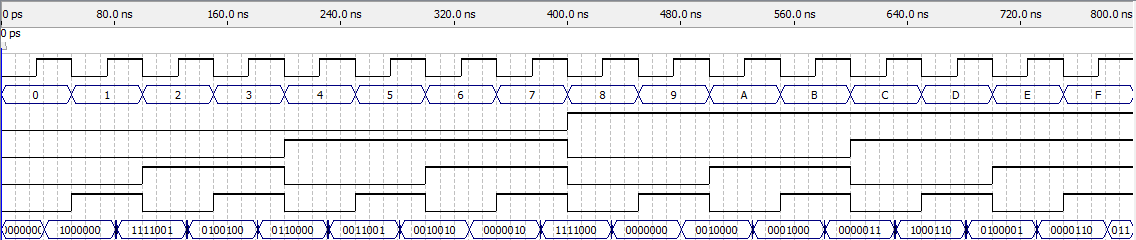
\includegraphics[width=.8\textwidth]{ex1_st.png}
	\caption{Simulação síncrona temporal do \textit{decoder7}.}
	\label{fig:ex1st}
\end{figure}

\begin{figure}[H]
	\centering
	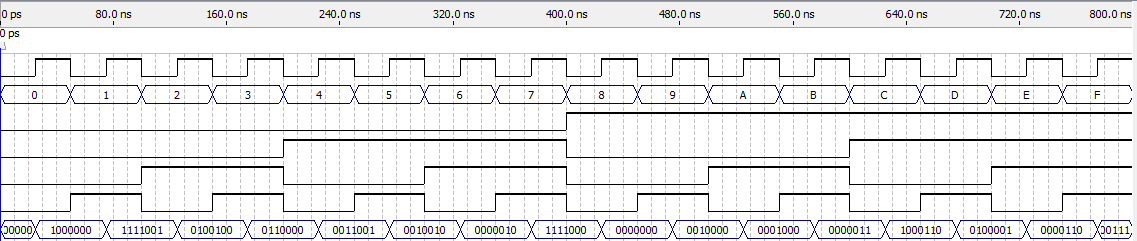
\includegraphics[width=.8\textwidth]{ex1_sf.png}
	\caption{Simulação síncrona funcional do \textit{decoder7}.}
	\label{fig:ex1sf}
\end{figure}

\begin{figure}[H]
	\centering
	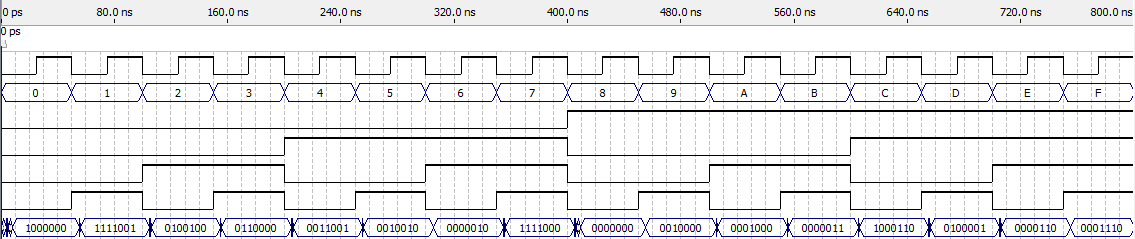
\includegraphics[width=.8\textwidth]{ex1_ast.png}
	\caption{Simulação assíncrona temporal do \textit{decoder7}.}
	\label{fig:ex1ast}
\end{figure}

\begin{figure}[H]
	\centering
	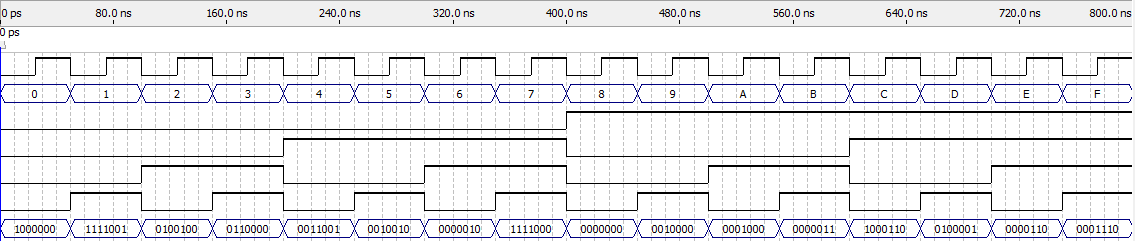
\includegraphics[width=.8\textwidth]{ex1_asf.png}
	\caption{Simulação assíncrona funcional do \textit{decoder7}.}
	\label{fig:ex1asf}
\end{figure}

O arquivo de interface \textit{TopDE.v} foi incluso no projeto, sintetizado e testado como é mostrado no link \url{https://youtu.be/wGKjze5PkcU}.

\subsection{Exercício 2. Unidade Lógica Aritmética de Inteiros}
\label{subsec:ulaint}

\subsubsection{Operações}
\label{subsubsec:2op}

% simulação temporal de cada operação
% usar valores comuns que gerem valores singulares (overflow, zero)
\begin{figure}[H]
	\centering
	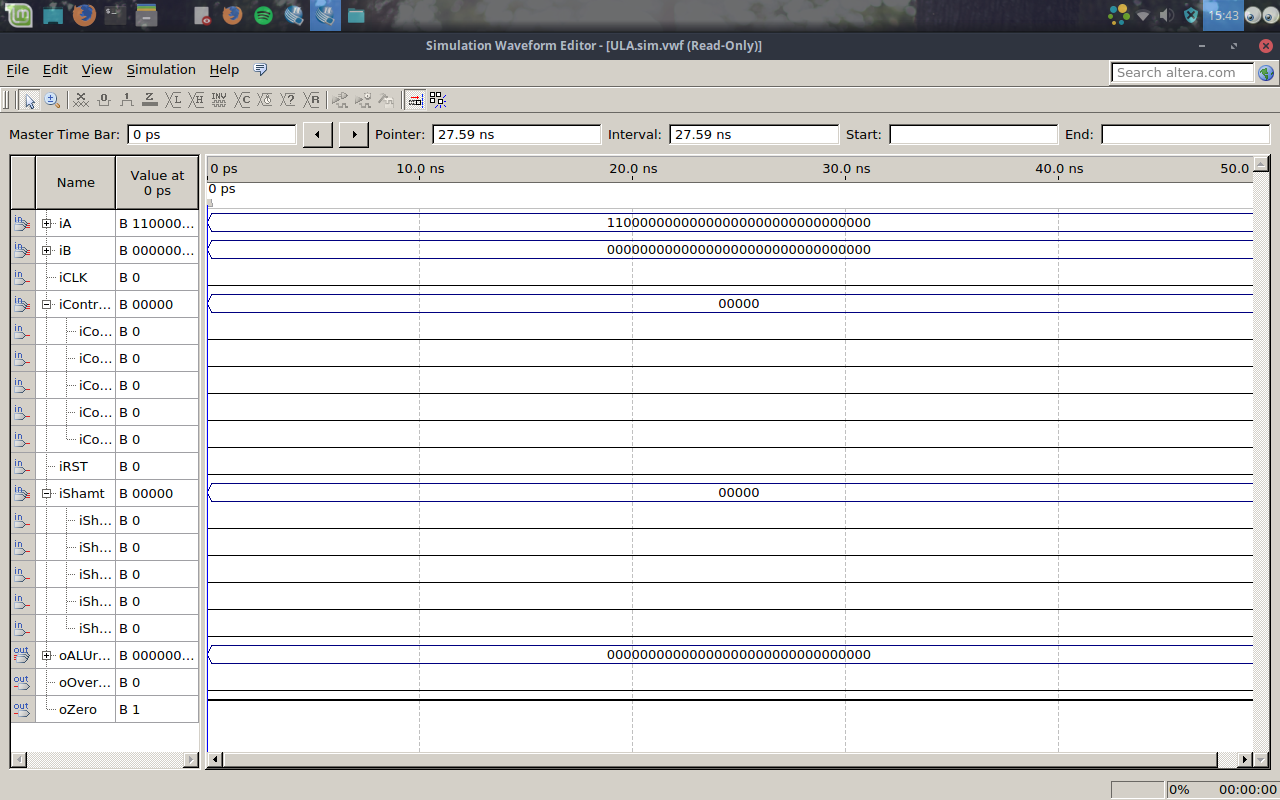
\includegraphics[width=.8\textwidth]{00000-and-zero.png}
	\caption{00000-and-zero}
	\label{fig:00000-and-zero}
\end{figure}

\begin{figure}[H]
	\centering
	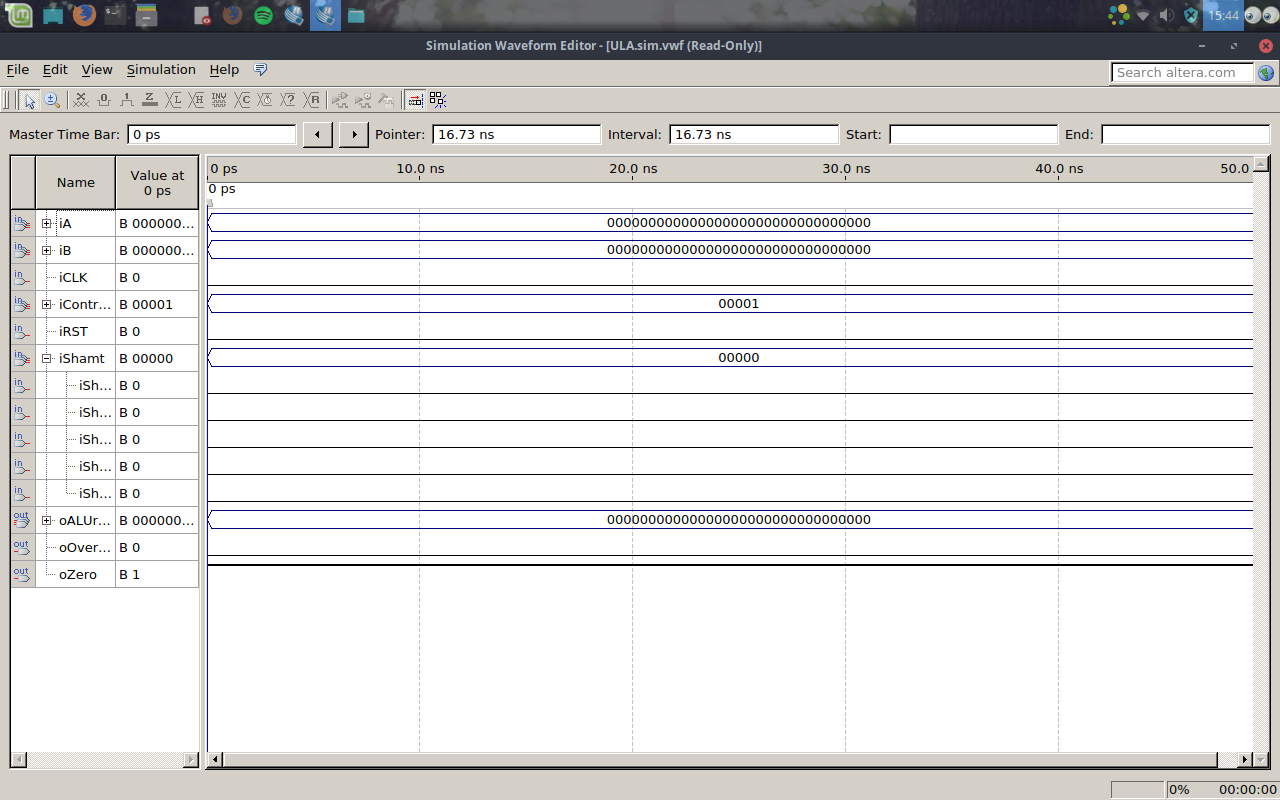
\includegraphics[width=.8\textwidth]{00001-or-zero.png}
	\caption{00001-or-zero}
	\label{fig:00001-or-zero}
\end{figure}

\begin{figure}[H]
	\centering
	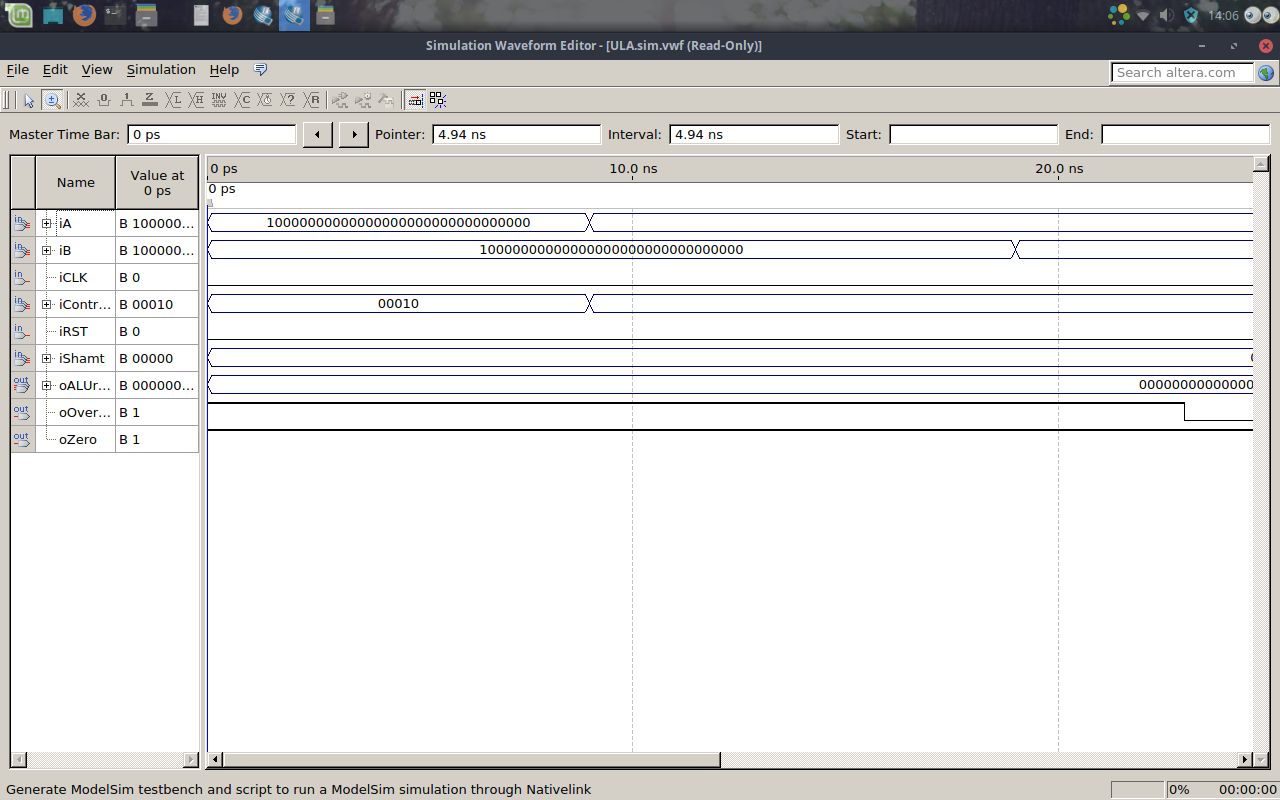
\includegraphics[width=.8\textwidth]{00010-add-over-zero.png}
	\caption{00010-add-over-zero}
	\label{fig:00010-add-over-zero}
\end{figure}

\begin{figure}[H]
	\centering
	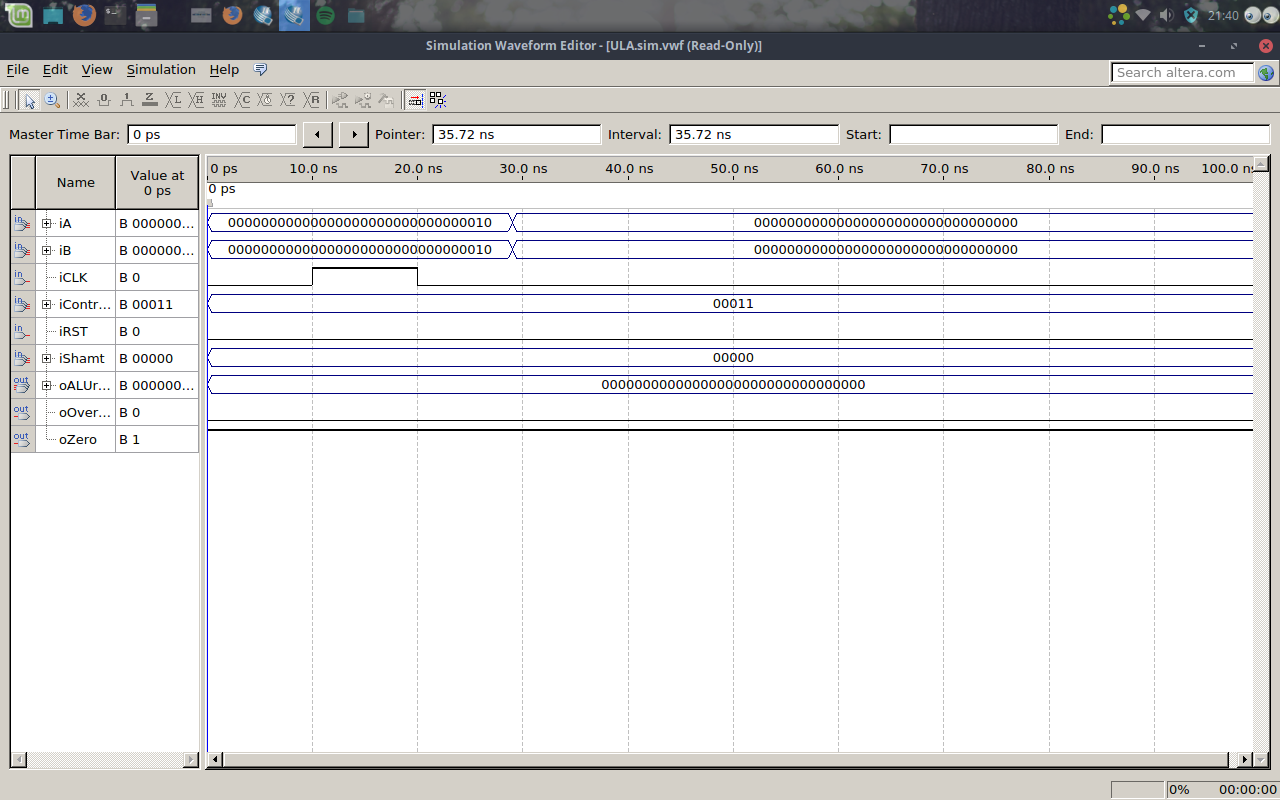
\includegraphics[width=.8\textwidth]{00011-mfhi-zero.png}
	\caption{00011-mfhi-zero}
	\label{fig:00011-mfhi-zero}
\end{figure}

\begin{figure}[H]
	\centering
	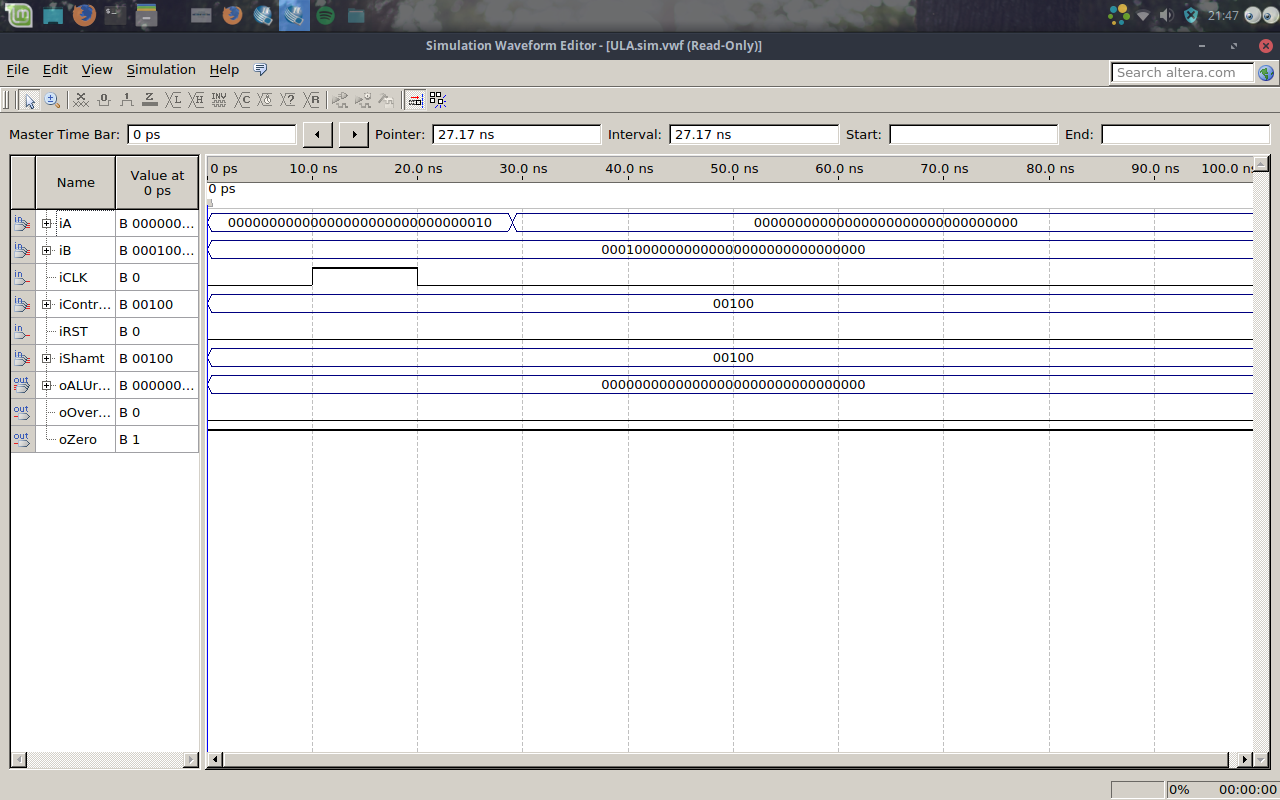
\includegraphics[width=.8\textwidth]{00100-sll-zero.png}
	\caption{00100-sll-zero}
	\label{fig:00100-sll-zero}
\end{figure}

\begin{figure}[H]
	\centering
	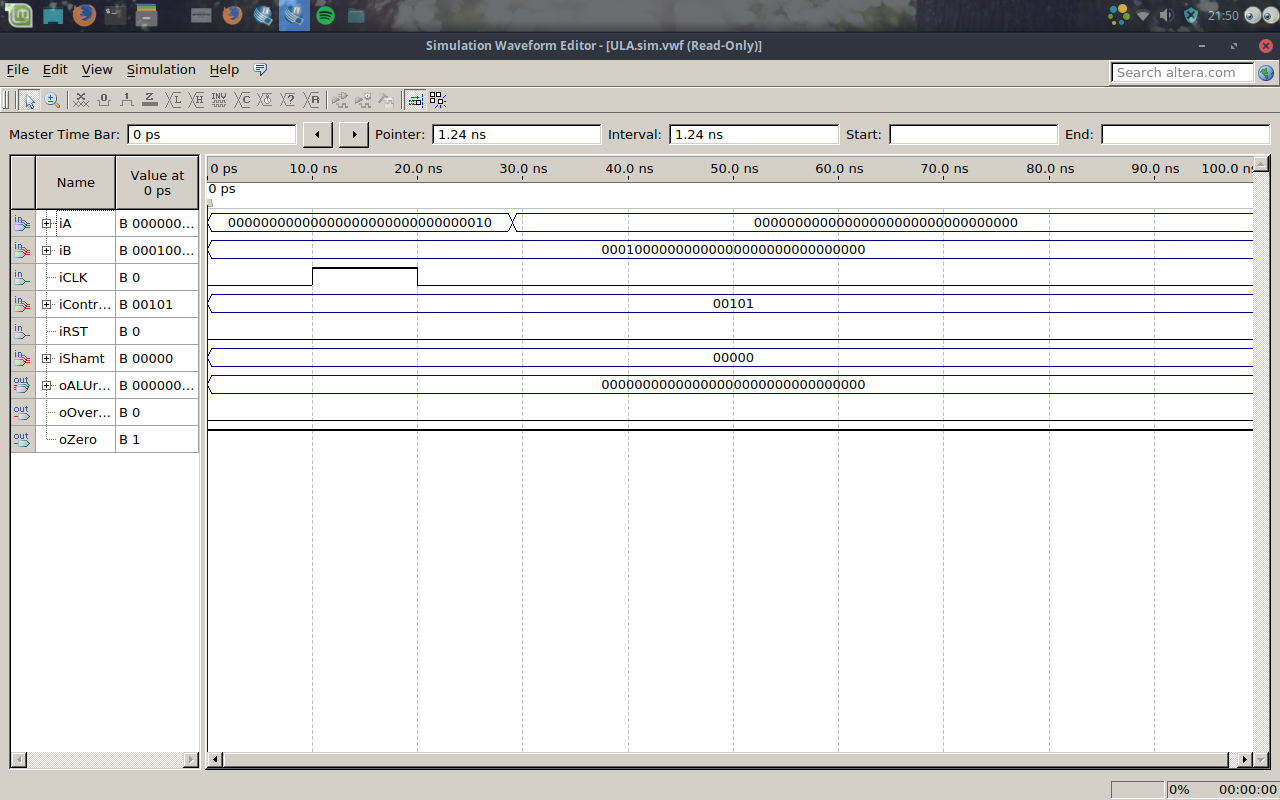
\includegraphics[width=.8\textwidth]{00101-mflo-zero.png}
	\caption{00101-mflo-zero}
	\label{fig:00101-mflo-zero}
\end{figure}

\begin{figure}[H]
	\centering
	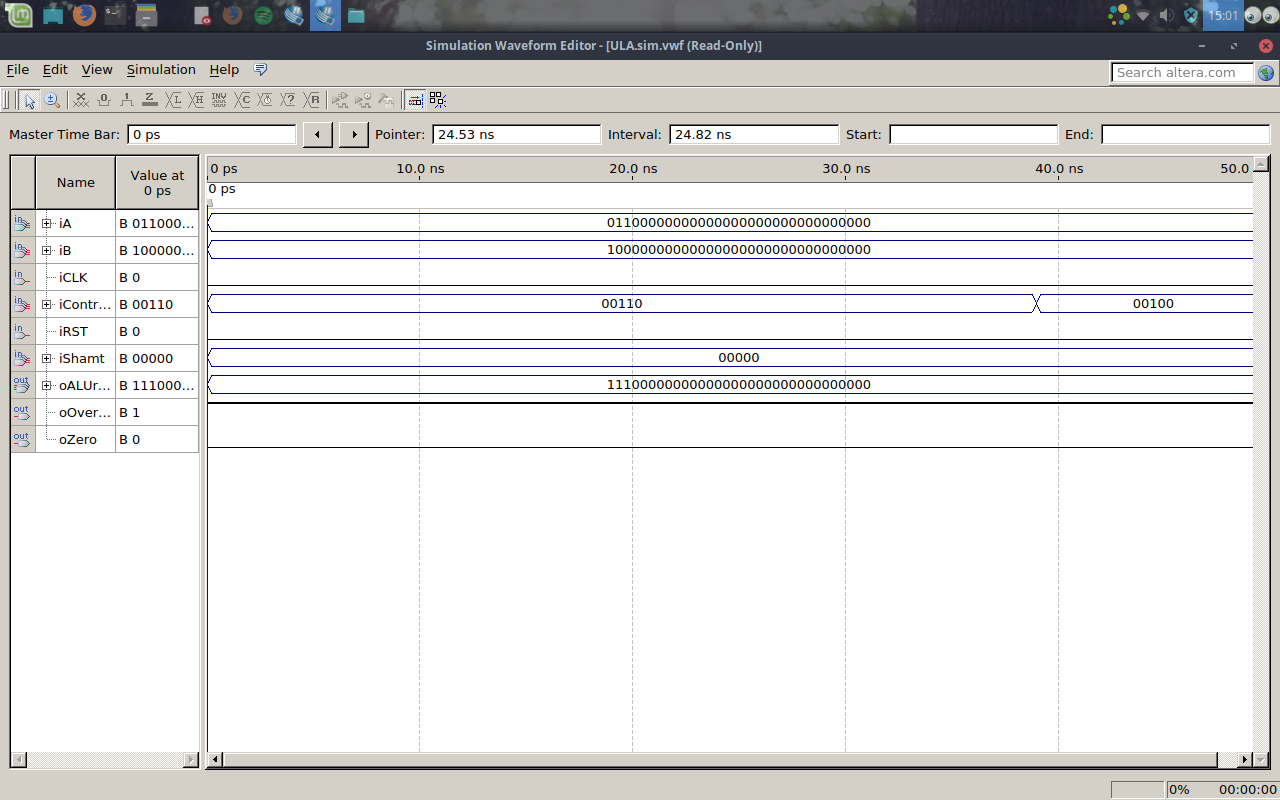
\includegraphics[width=.8\textwidth]{00110-sub-over.png}
	\caption{00110-sub-over}
	\label{fig:00110-sub-over}
\end{figure}

\begin{figure}[H]
	\centering
	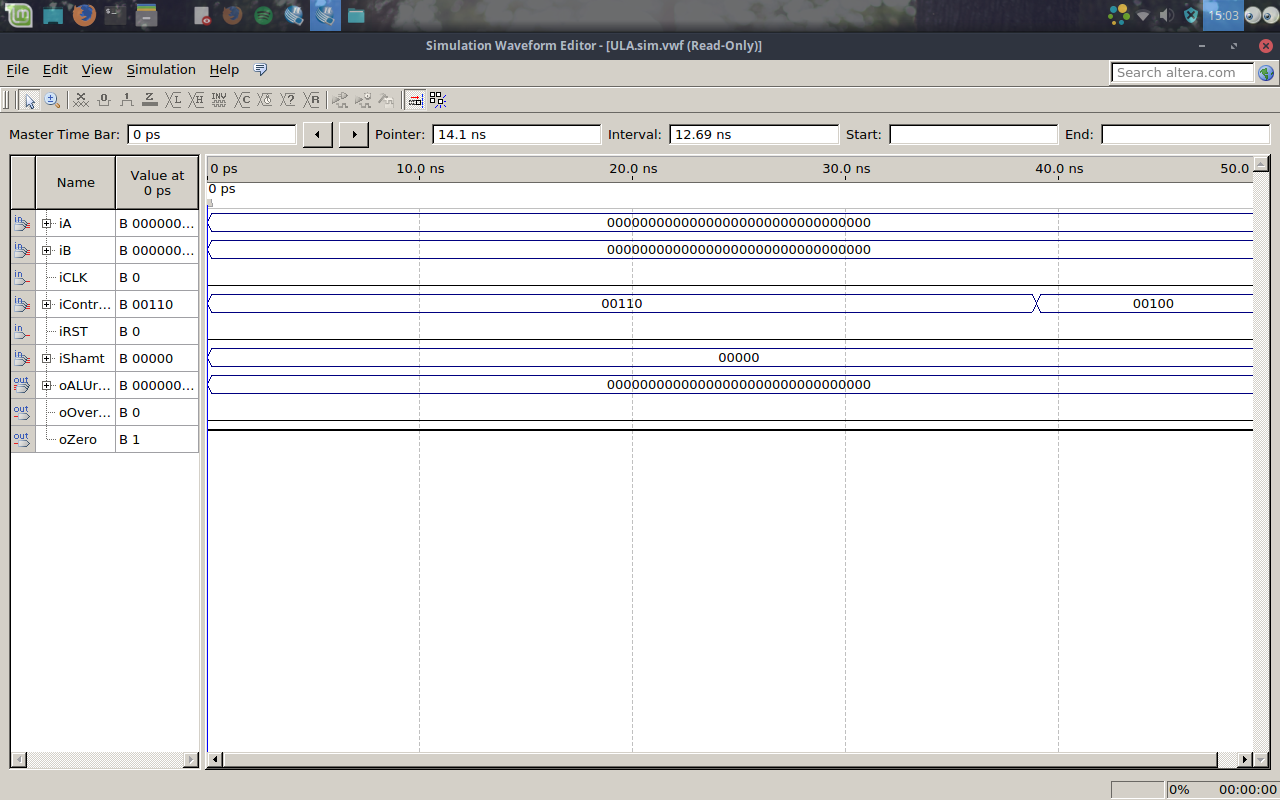
\includegraphics[width=.8\textwidth]{00110-sub-zero.png}
	\caption{00110-sub-zero}
	\label{fig:00110-sub-zero}
\end{figure}

\begin{figure}[H]
	\centering
	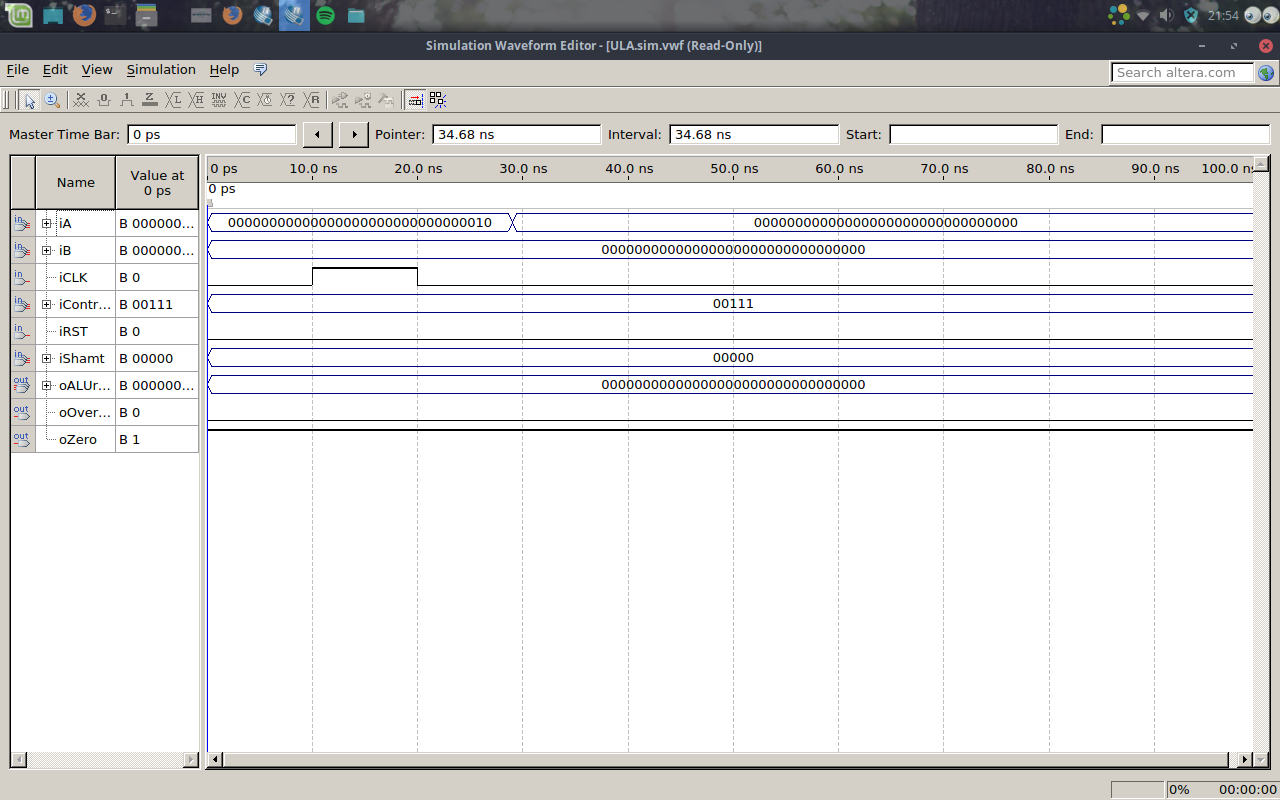
\includegraphics[width=.8\textwidth]{00111-slt-zero.png}
	\caption{00111-slt-zero}
	\label{fig:00111-slt-zero}
\end{figure}

\begin{figure}[H]
	\centering
	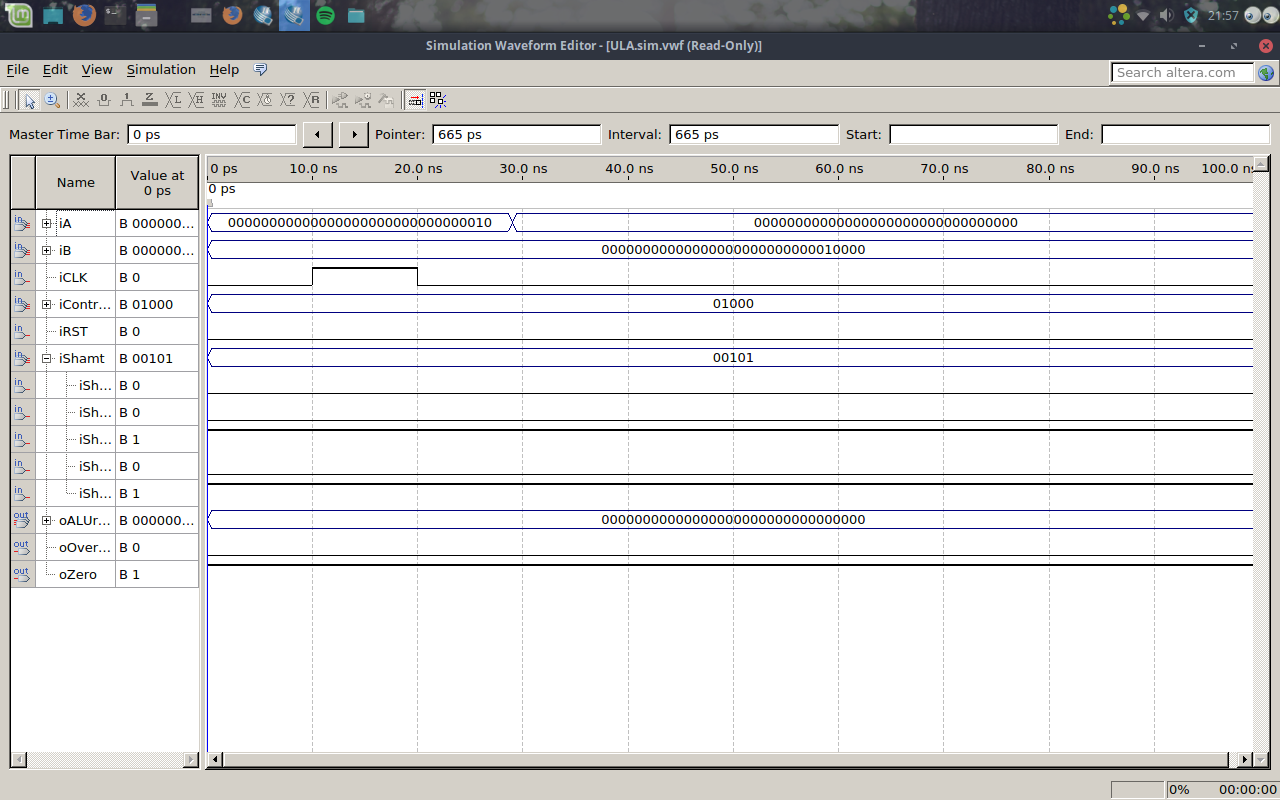
\includegraphics[width=.8\textwidth]{01000-srl-zero.png}
	\caption{01000-srl-zero}
	\label{fig:01000-srl-zero}
\end{figure}

\begin{figure}[H]
	\centering
	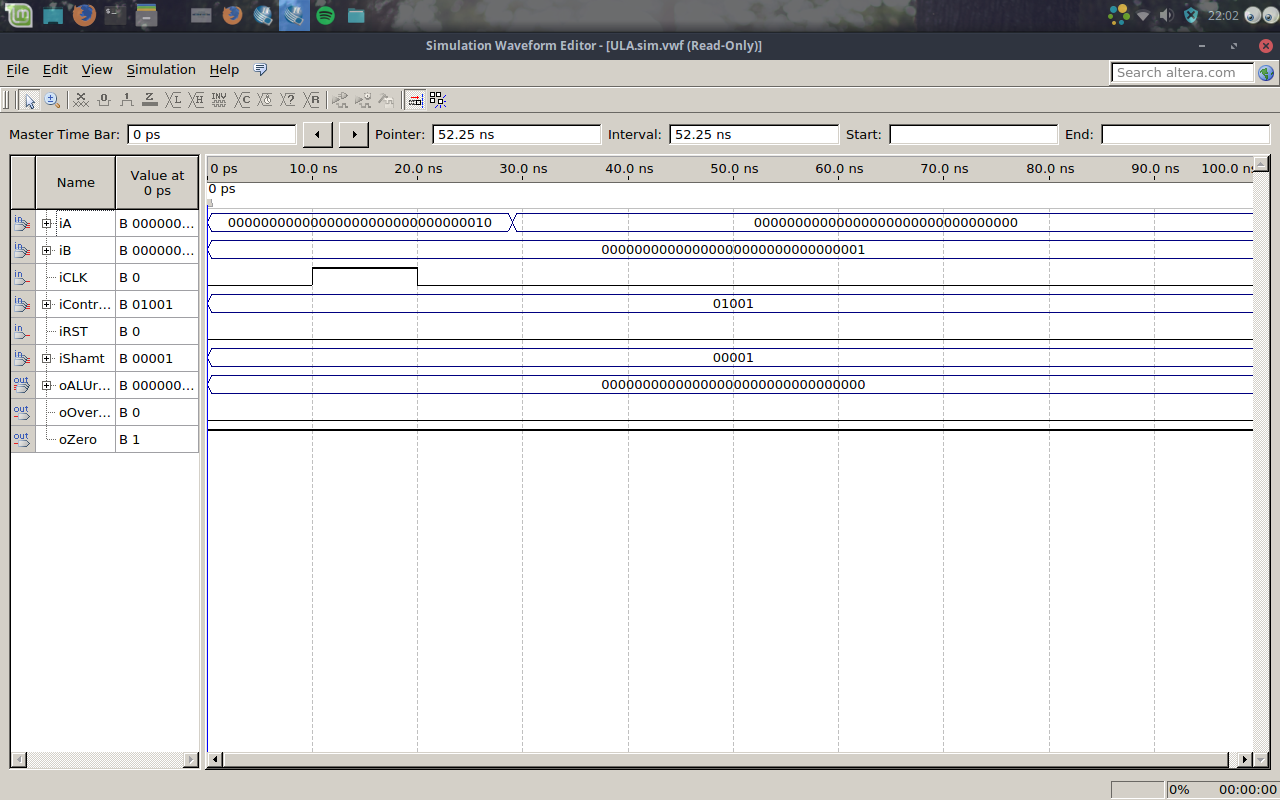
\includegraphics[width=.8\textwidth]{01001-sra-zero.png}
	\caption{01001-sra-zero}
	\label{fig:01001-sra-zero}
\end{figure}

\begin{figure}[H]
	\centering
	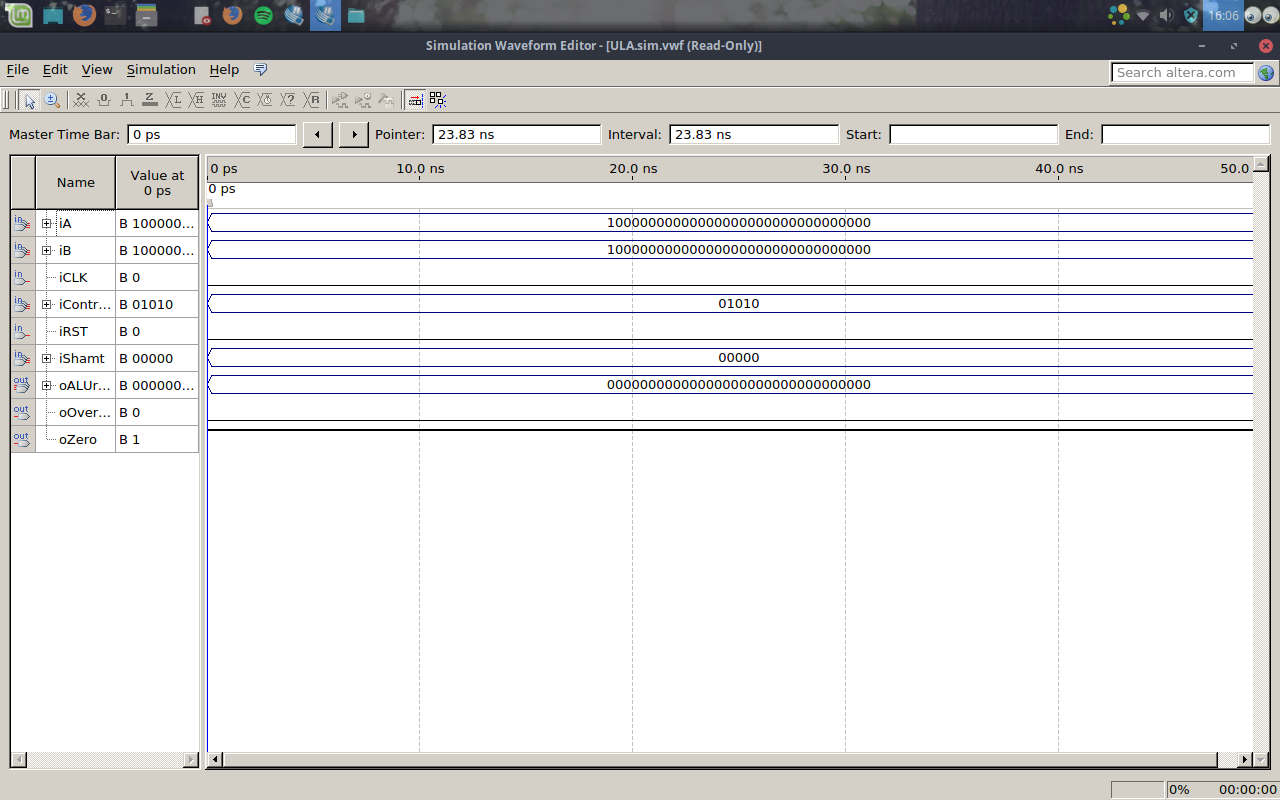
\includegraphics[width=.8\textwidth]{01010-xor-zero.png}
	\caption{01010-xor-zero}
	\label{fig:01010-xor-zero}
\end{figure}

\begin{figure}[H]
	\centering
	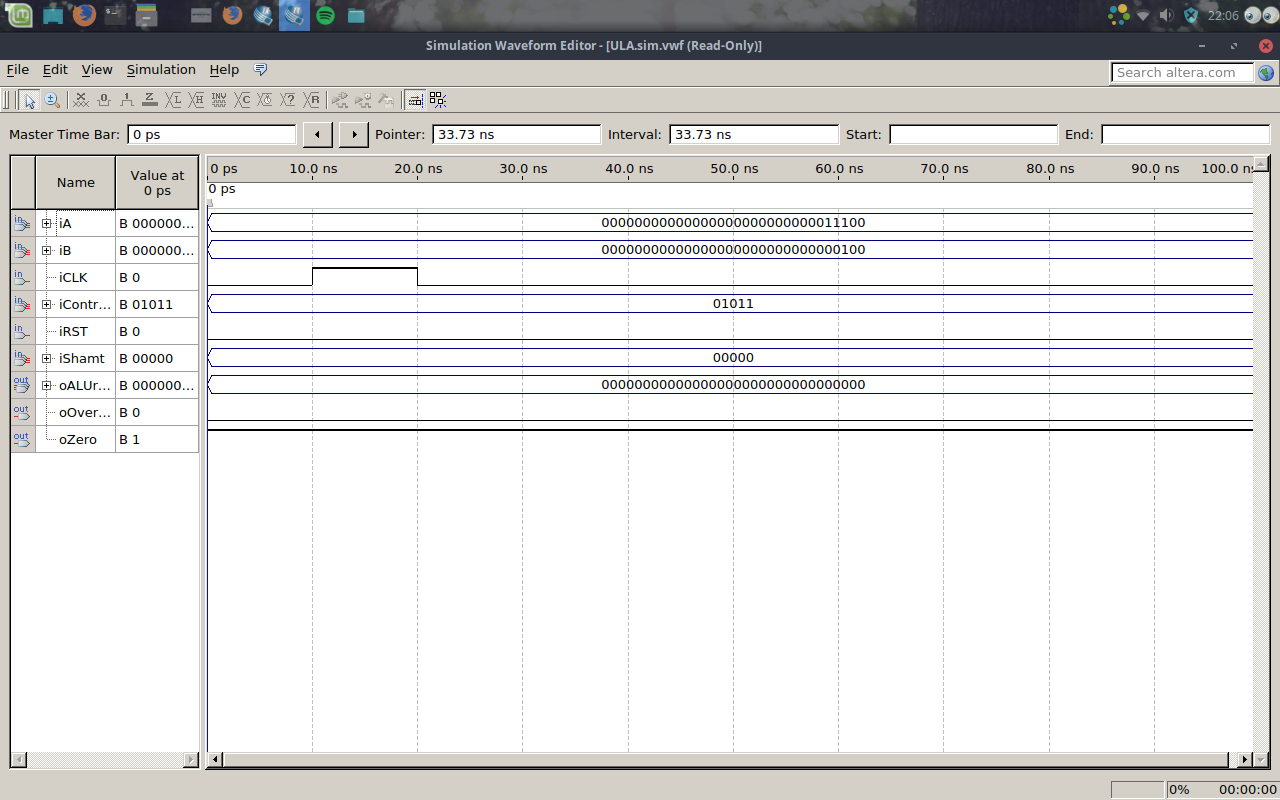
\includegraphics[width=.8\textwidth]{01011-sltu-zero.png}
	\caption{01011-sltu-zero}
	\label{fig:01011-sltu-zero}
\end{figure}

\begin{figure}[H]
	\centering
	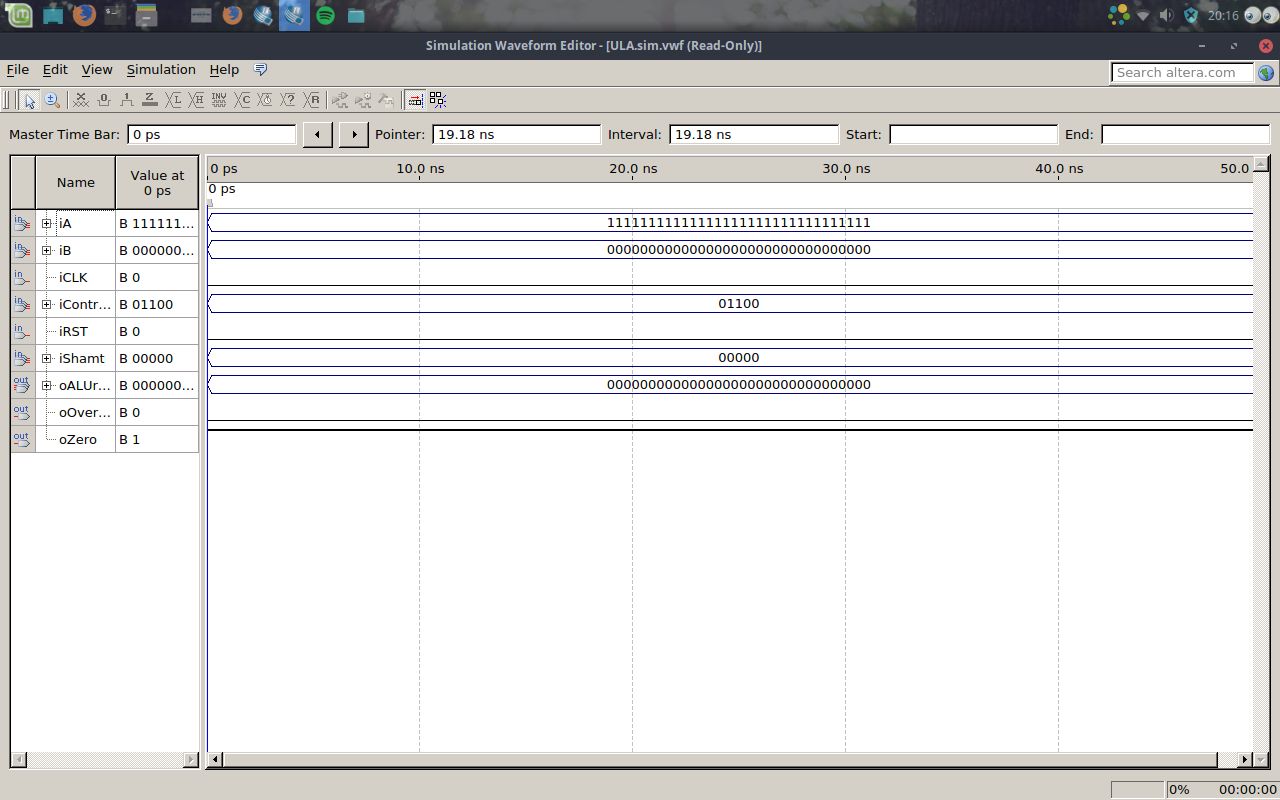
\includegraphics[width=.8\textwidth]{01100-nor-zero.png}
	\caption{01100-nor-zero}
	\label{fig:01100-nor-zero}
\end{figure}

\begin{figure}[H]
	\centering
	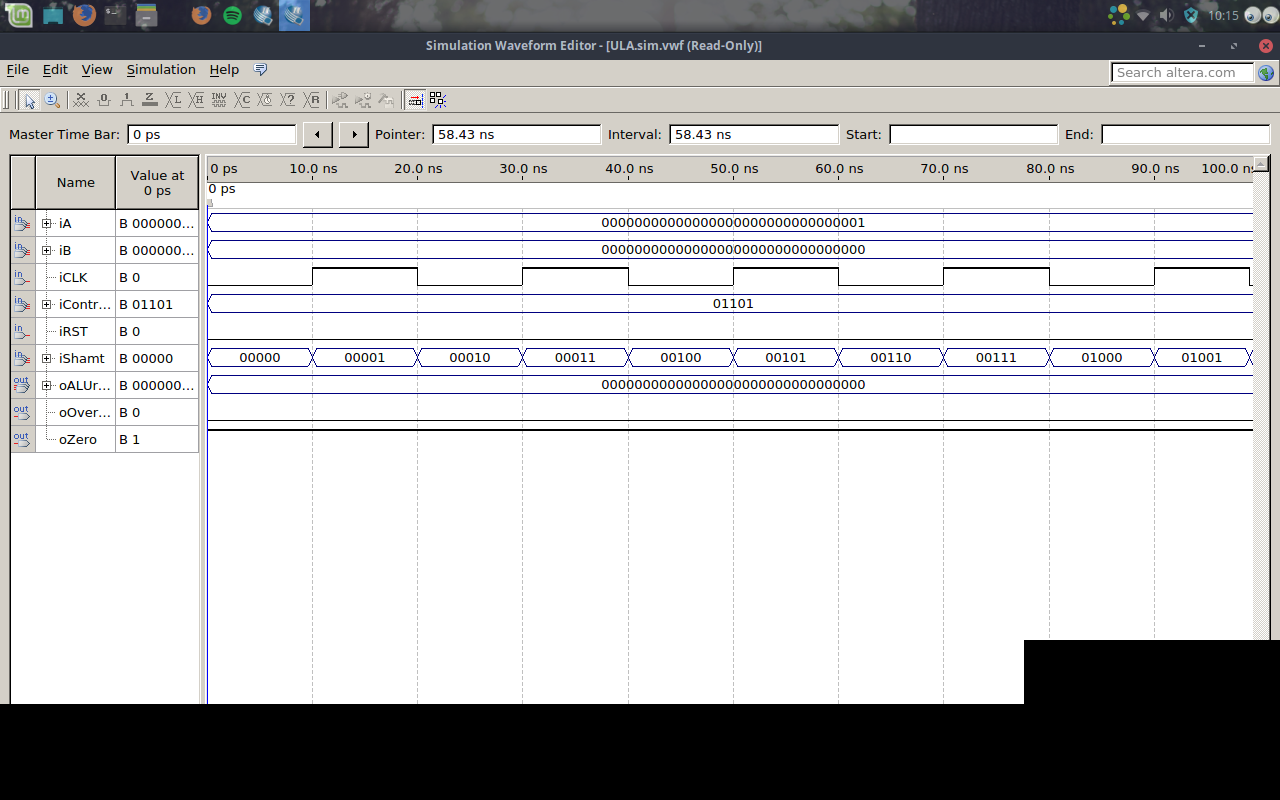
\includegraphics[width=.8\textwidth]{01101-mult-zero.png}
	\caption{01101-mult-zero}
	\label{fig:01101-mult-zero}
\end{figure}

\begin{figure}[H]
	\centering
	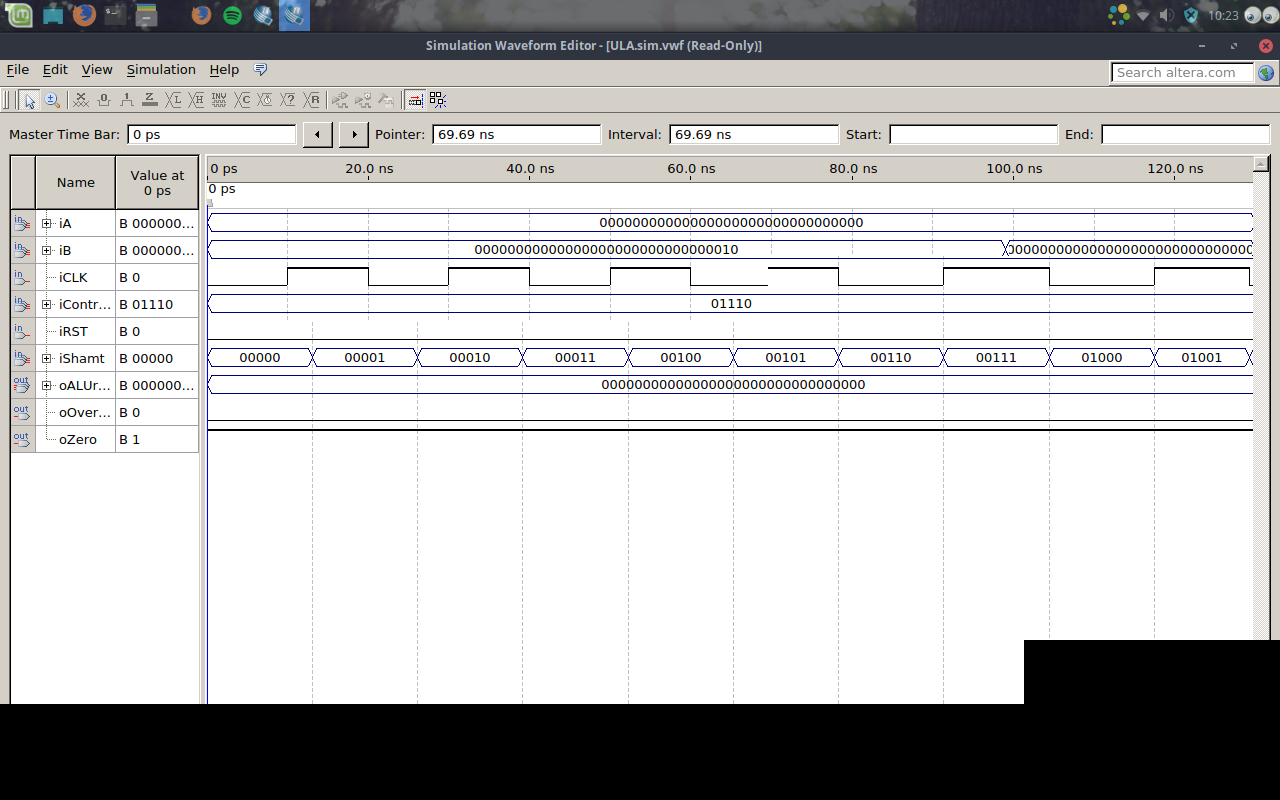
\includegraphics[width=.8\textwidth]{01110-div-zero.png}
	\caption{01110-div-zero}
	\label{fig:01110-div-zero}
\end{figure}

\begin{figure}[H]
	\centering
	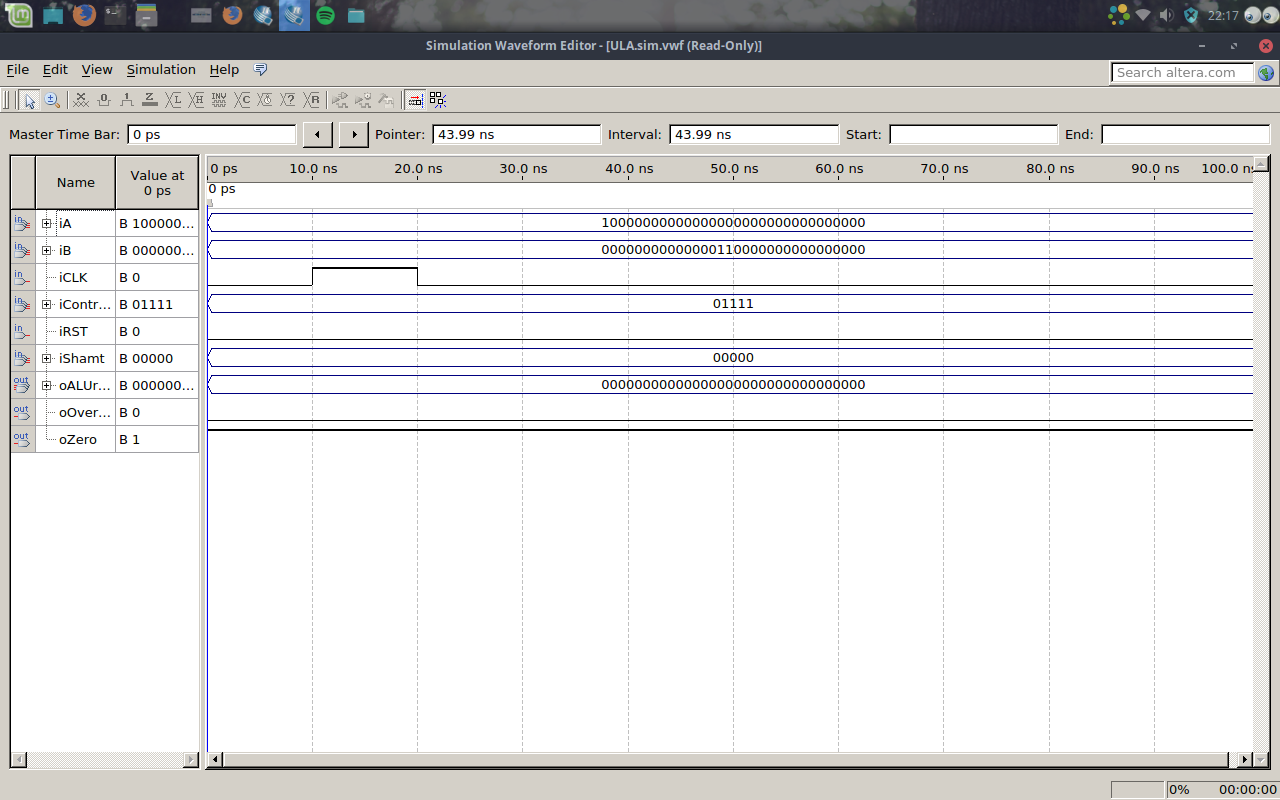
\includegraphics[width=.8\textwidth]{01111-lui-zero.png}
	\caption{01111-lui-zero}
	\label{fig:01111-lui-zero}
\end{figure}

\begin{figure}[H]
	\centering
	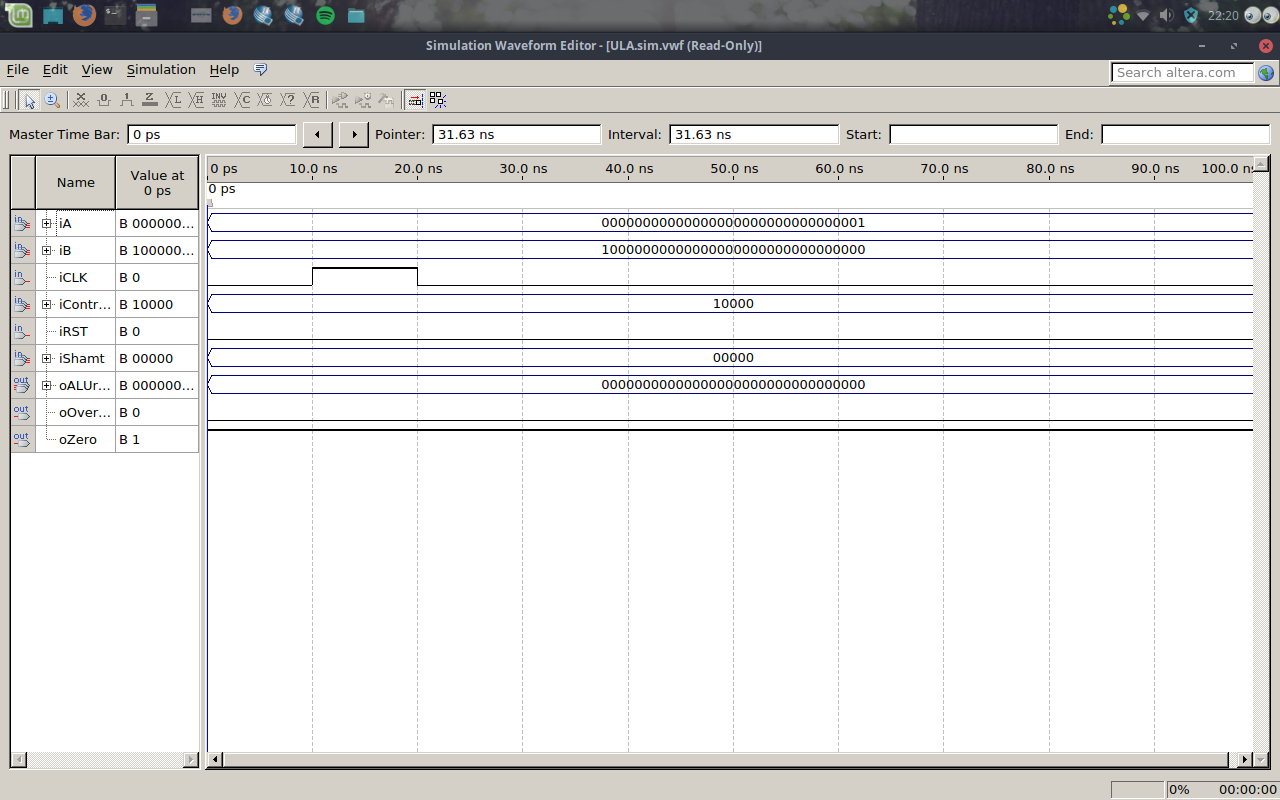
\includegraphics[width=.8\textwidth]{10000-sllv-zero.png}
	\caption{10000-sllv-zero}
	\label{fig:10000-sllv-zero}
\end{figure}

\begin{figure}[H]
	\centering
	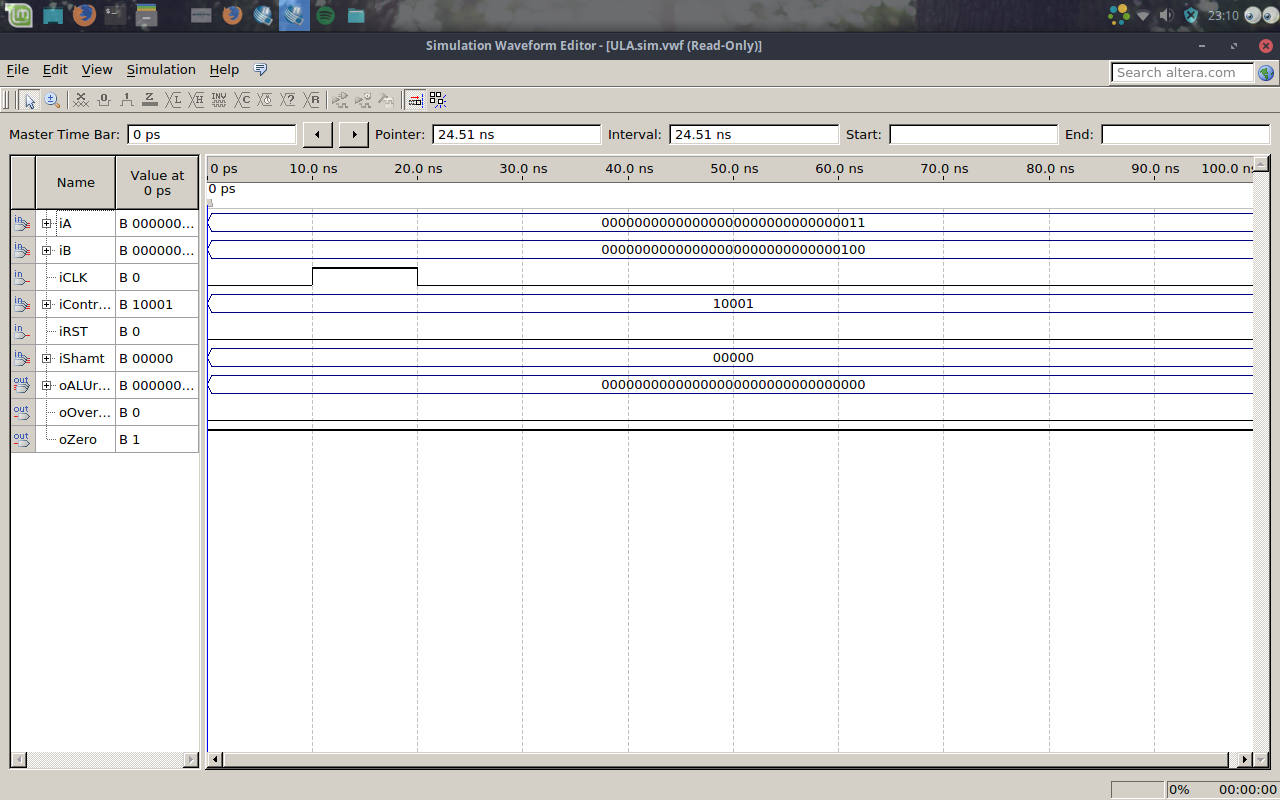
\includegraphics[width=.8\textwidth]{10001-srav-zero.png}
	\caption{10001-srav-zero}
	\label{fig:10001-srav-zero}
\end{figure}

\begin{figure}[H]
	\centering
	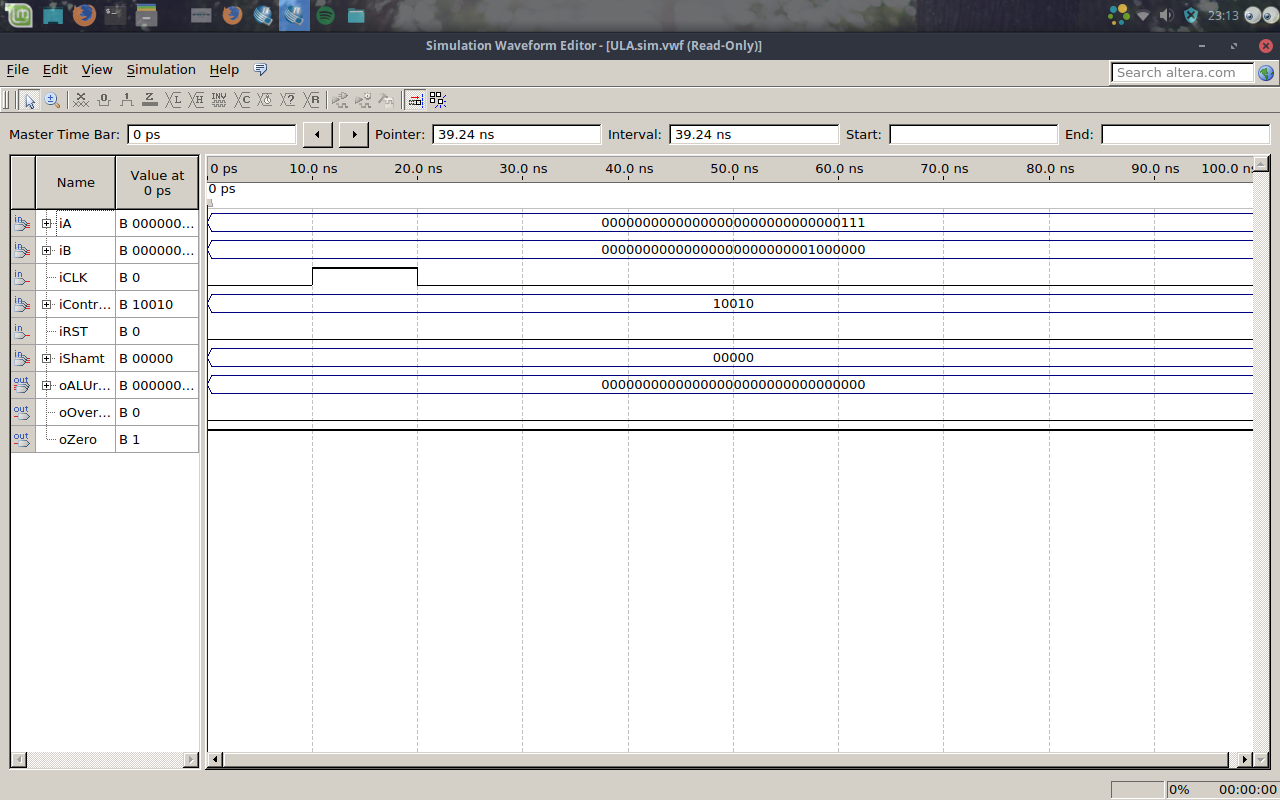
\includegraphics[width=.8\textwidth]{10010-srlv-zero.png}
	\caption{10010-srlv-zero}
	\label{fig:10010-srlv-zero}
\end{figure}

\begin{figure}[H]
	\centering
	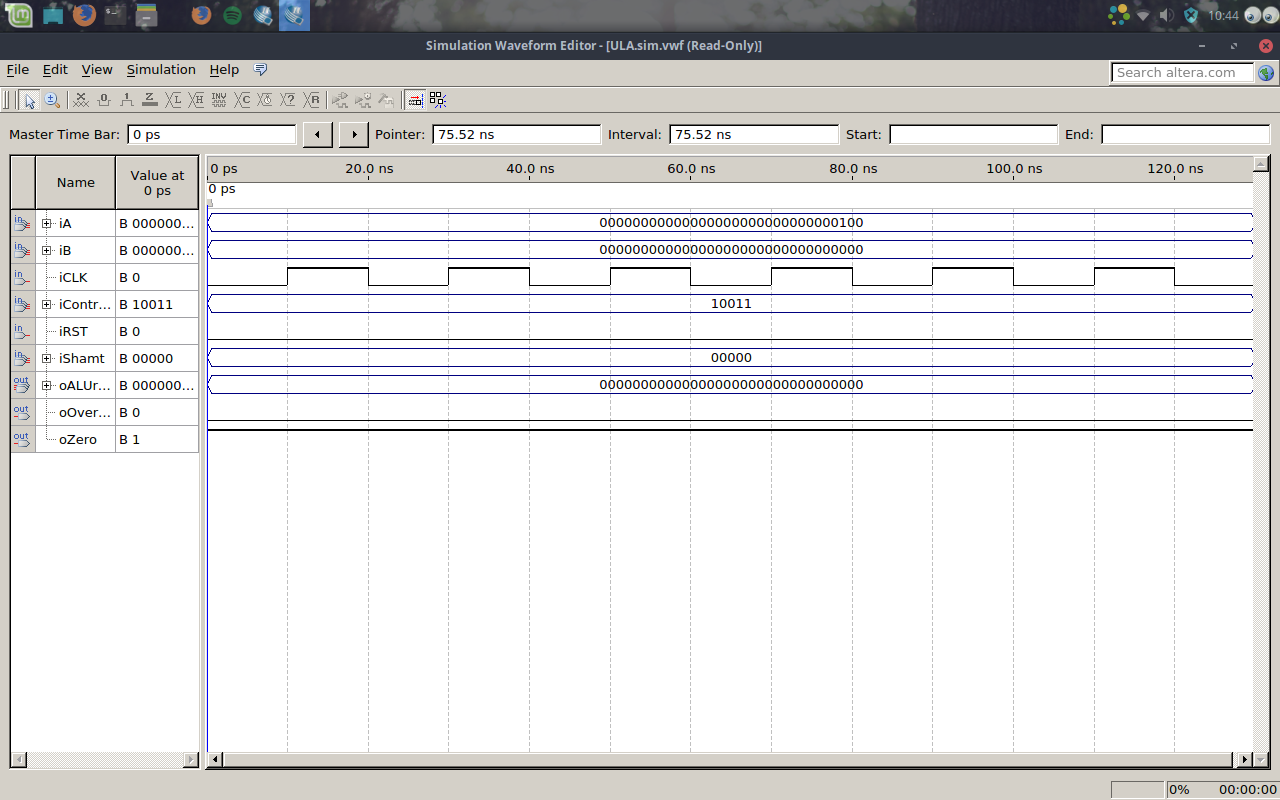
\includegraphics[width=.8\textwidth]{10011-multu-zero.png}
	\caption{10011-multu-zero}
	\label{fig:10011-multu-zero}
\end{figure}

\begin{figure}[H]
	\centering
	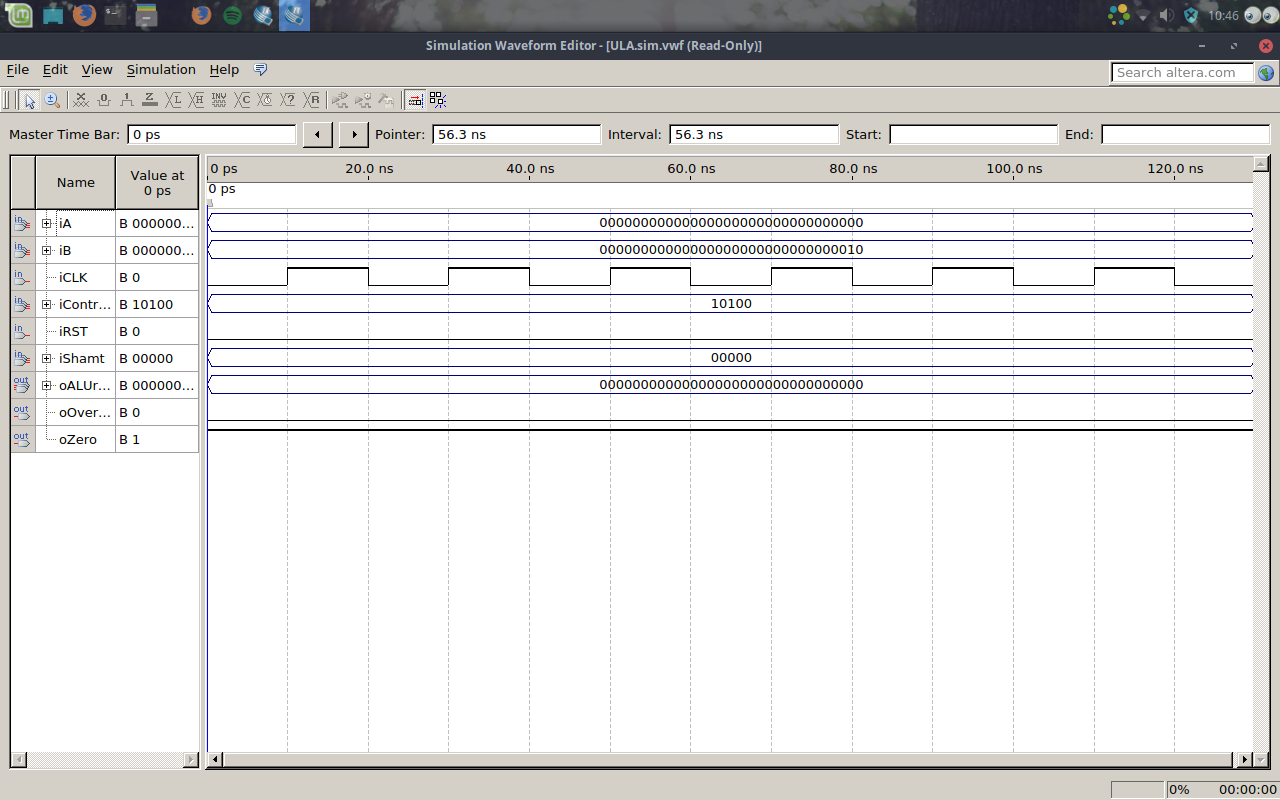
\includegraphics[width=.8\textwidth]{10100-divu-zero.png}
	\caption{10100-divu-zero}
	\label{fig:10100-divu-zero}
\end{figure}

\begin{figure}[H]
	\centering
	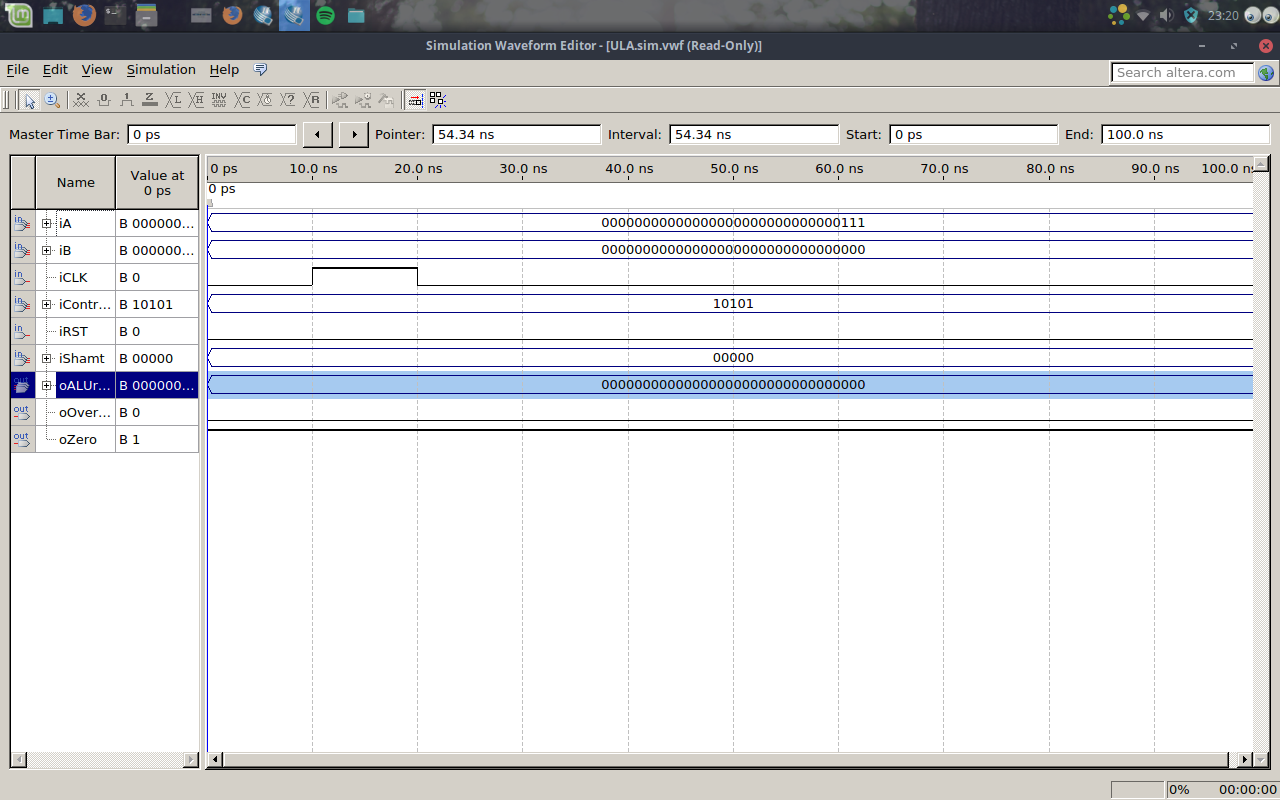
\includegraphics[width=.8\textwidth]{10101-mthi-zero.png}
	\caption{10101-mthi-zero}
	\label{fig:10101-mthi-zero}
\end{figure}

\begin{figure}[H]
	\centering
	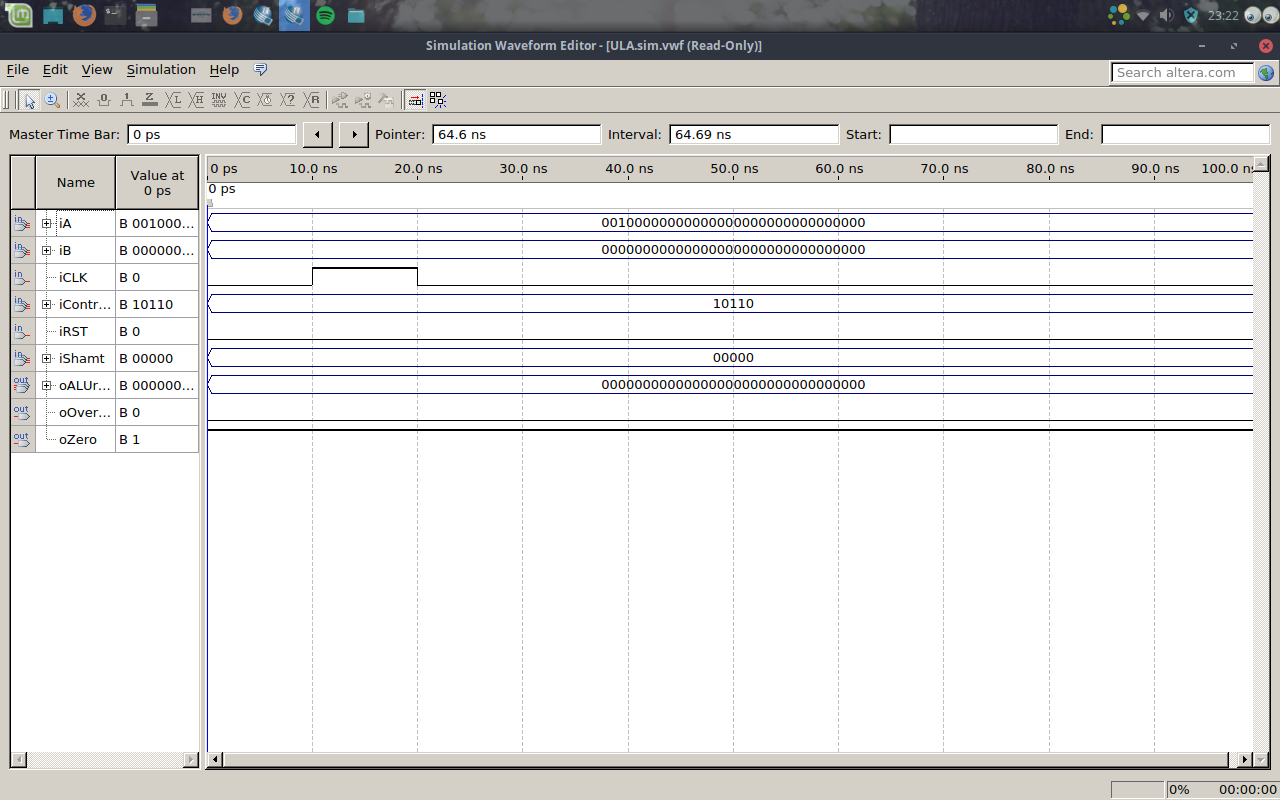
\includegraphics[width=.8\textwidth]{10110-mtlo-zero.png}
	\caption{10110-mtlo-zero}
	\label{fig:10110-mtlo-zero}
\end{figure}

\begin{figure}[H]
	\centering
	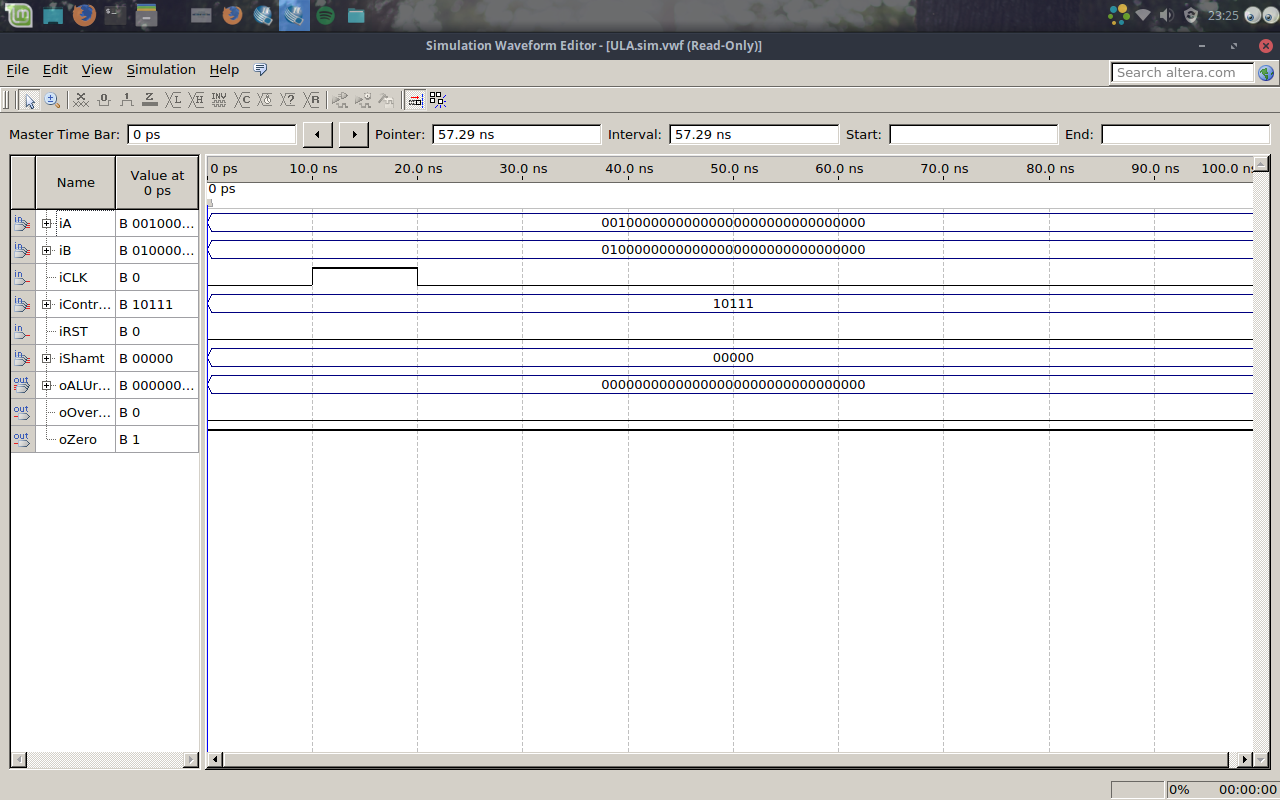
\includegraphics[width=.8\textwidth]{10111-sgt-zero.png}
	\caption{10111-sgt-zero}
	\label{10111-sgt-zero}
\end{figure}

\begin{figure}[H]
	\centering
	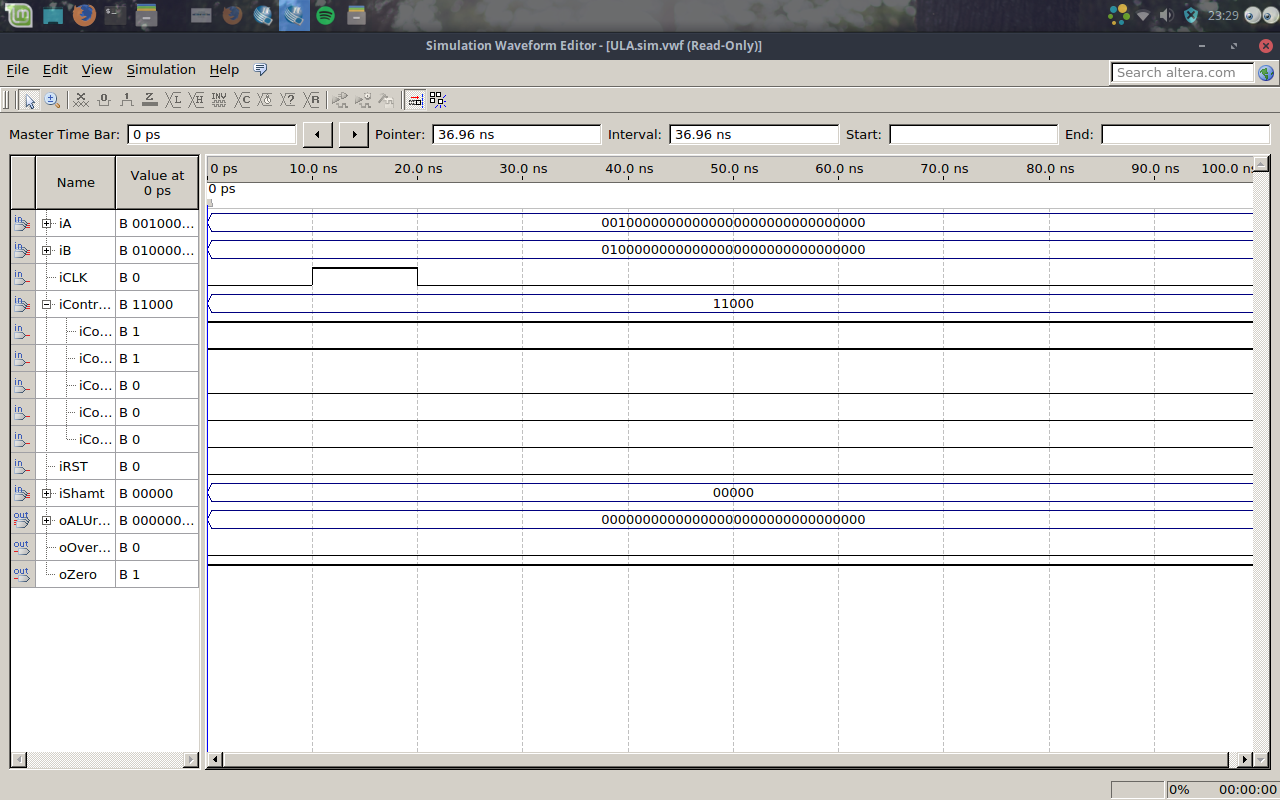
\includegraphics[width=.8\textwidth]{11000-madd-zero.png}
	\caption{11000-madd-zero}
	\label{fig:11000-madd-zero}
\end{figure}

\begin{figure}[H]
	\centering
	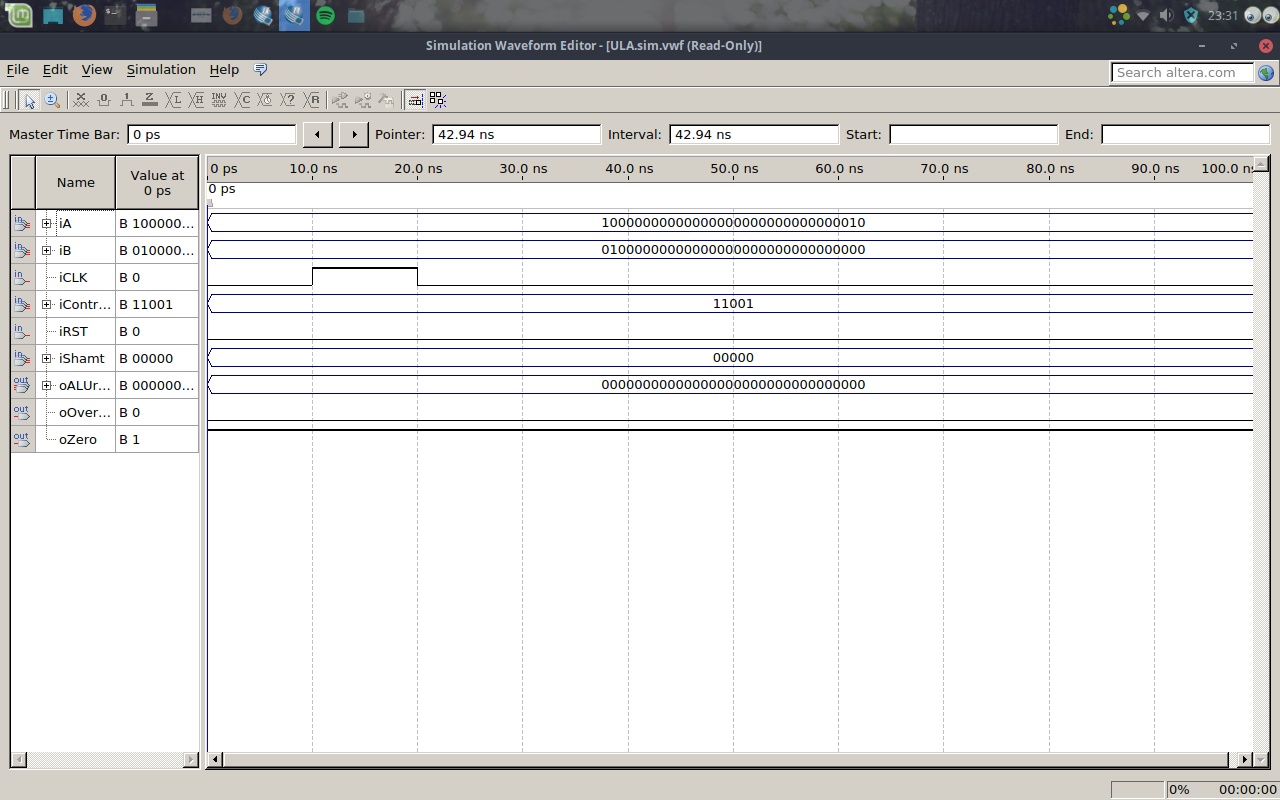
\includegraphics[width=.8\textwidth]{11001-maddu-zero.png}
	\caption{11001-maddu-zero}
	\label{fig:11001-maddu-zero}
\end{figure}

\begin{figure}[H]
	\centering
	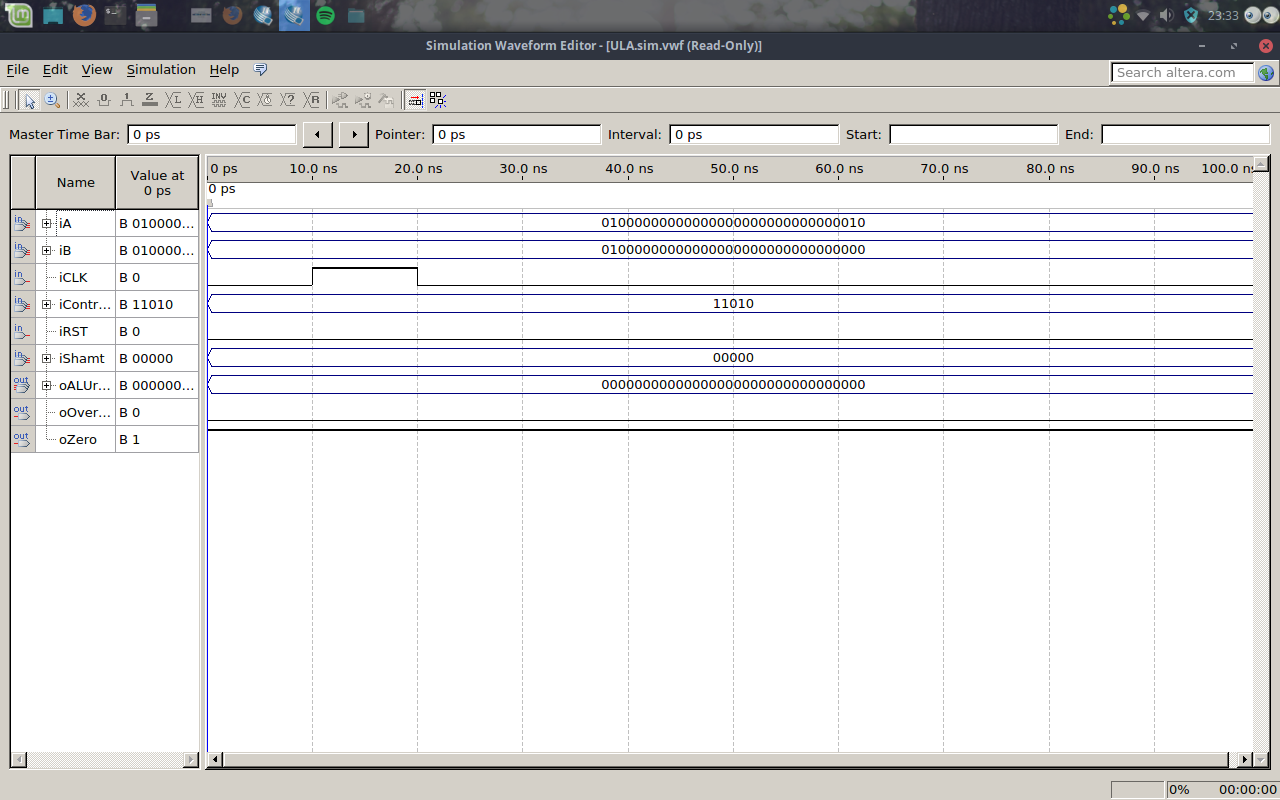
\includegraphics[width=.8\textwidth]{11010-msub-zero.png}
	\caption{11010-msub-zero}
	\label{fig:11010-msub-zero}
\end{figure}

\begin{figure}[H]
	\centering
	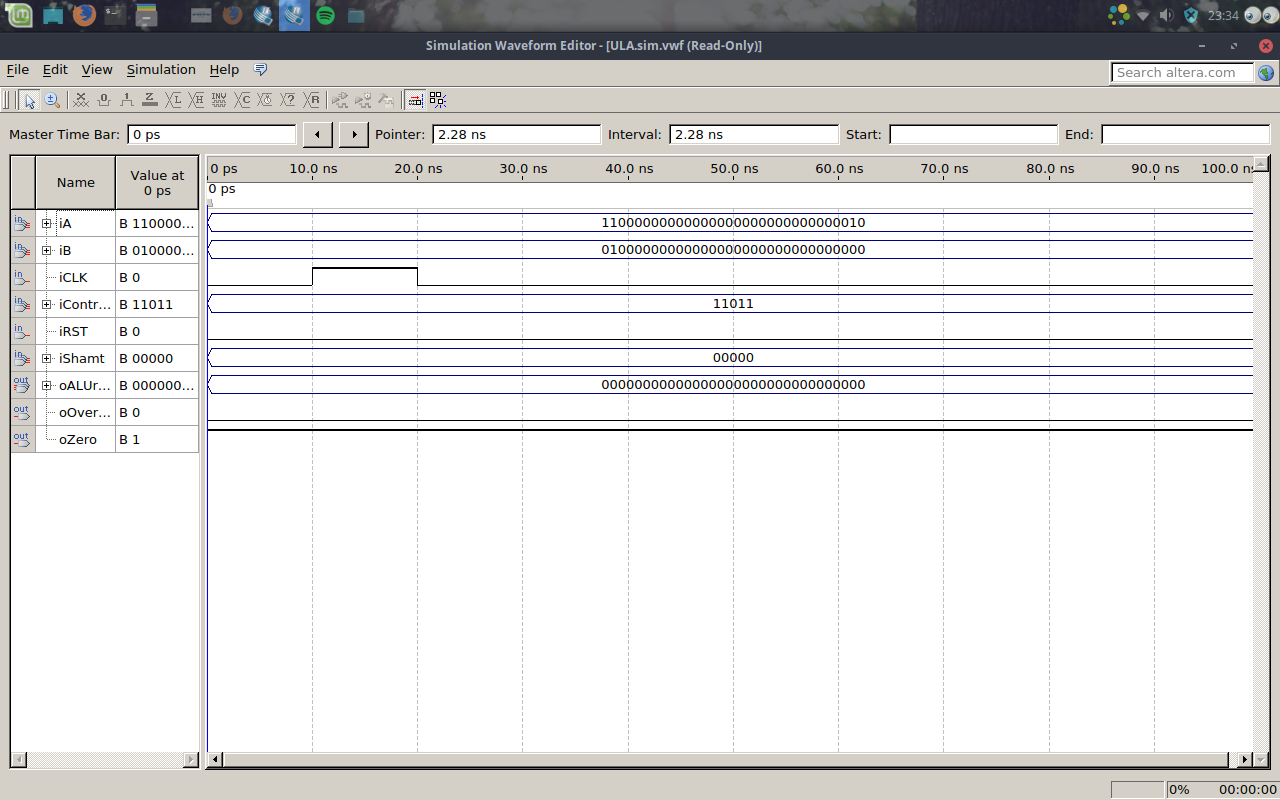
\includegraphics[width=.8\textwidth]{11011-msubu-zero.png}
	\caption{11011-msubu-zero}
	\label{fig:11011-msubu-zero}
\end{figure}



\subsubsection{Requisitos físicos}
\label{subsubsec:ulafis}

Para a ULA de inteiros foi levantado os requisitos físicos de cada operação e da ULA total como podemos ver na Tabela~\ref{tab:req21} e Tabela~\ref{tab:req22}. Todos estes dados foram encontrados utilizando o seguinte procedimento:

\begin{itemize}
	\item Foi aberto o projeto da \textit{ULA} no \textit{Quartus II 64-Bit};
	\item No arquivo \textit{ALU.v} para testar a ULA completa foi preciso comentar as linhas "\textit{wire [4:0]  iControlSignal}" e "\textit{assign iControlSignal=OPMSUB}" e descomentar a linha "\textit{input [4:0] iControlSignal}". No arquivo \textit{ALU.v} para testar cada operação foi preciso descomentar as linhas "\textit{wire [4:0]  iControlSignal}" e "\textit{assign iControlSignal=OPMSUB}" e comentar a linha "\textit{input [4:0] iControlSignal}". A troca de operação avaliada foi feita substituindo o nome da operação na variável \textit{iControlSignal} (e.g. assign iControlSignal=OPSLL);
	\item Ao trocar a operação desejada foi compilado o projeto;
	\item Com a nova aba (\textit{Compilation Report - ULA}) aberta, no menu \textit{Flow Summary} foi possível achar informações da quantidade total de elementos lógicos usado naquela operação;
	\item No menu \textit{TimeQuest Timing Analyzer $>$ Multicorner Datasheet Report Summary} foram encontrados valores dos maiores / menores tempos de atraso para concluir a operação. Estes tempos são medidos desde o ato de inserir o dado na entrada (\textit{iA} e/ou \textit{iB}) e resultar em algo na saída (\textit{oALUresult}). Alguns resultados assíncronos eram aparentes na aba \textit{RR} (medição ao subir a borda inicial até a subida da borda final), outros na \textit{RF} (medição ao subir a borda inicial até a descida da borda final) \cite{altera}. Para operações síncronas era possível captar os resultados na aba \textit{Rise};
		\begin{itemize}
			\item Para operações puramente assíncronas o maior tempo foi encontrado no menu \textit{Propagation Delay}. Para operações também síncronas tiveram estes dados aparentes no menu \textit{Clock to Output Times}; 
			\item Para operações puramente assíncronas o menor tempo foi encontrado no menu \textit{Minimum Propagation Delay}. Para operações também síncronas tiveram estes dados aparentes no menu \textit{Minimum Clock to Output Times}. 
		\end{itemize}
	\item A frequência máxima de \textit{clock} utilizável foi gerada a partir do cálculo $F_{MAX} = 1/T$, sendo $T$ o maior tempo de atraso da operação. Esse $T$ tem que ser o pior caso de tempo ocorrido pois precisa ser suficiente para concluir toda a operação em qualquer caso.
\end{itemize}

\begin{table}[H]
	\centering
	\begin{tabular}{|c|c|c|c|c|}
		\hline
		& \textbf{Elementos} & \textbf{Menor} & \textbf{Maior} & \textbf{Frequência máxima de} \\
		& \textbf{lógicos} & \textbf{atraso (ns)} &  \textbf{atraso (ns)} & \textbf{\textit{clock} utilizável (MHz)} \\
		\hline
		\textbf{ULA} & 6686 & 4,788 & 26,648 & 37,526 \\\hline
		\textbf{OPAND} & 43 & 5,495 & 9,810 & 101,937 \\\hline
		\textbf{OPOR} & 43 & 5,490 & 9,811 & 101,926 \\\hline
		\textbf{OPADD} & 44 & 5,081 & 14,134 & 70,751 \\\hline
		\textbf{OPMFHI} & 0 & 0 & 0 & 0 \\\hline
		\textbf{OPSLL} & 170 & 6,000 & 15,048 & 66,454 \\\hline
		\textbf{OPMFLO} & 0 & 0 & 0 & 0 \\\hline
		\textbf{OPSUB} & 44 & 5,119 & 13,909 & 71,896 \\\hline
		\textbf{OPSLT} & 32 & 5,341 & 13,470 & 74,239 \\\hline
		\textbf{OPSGT} & 32 & 5,341 & 13,470 & 74,239 \\\hline
		\textbf{OPSRL} & 170 & 6,065 & 16,137 & 61,969 \\\hline
		\textbf{OPSRA} & 174 & 4,908 & 15,736 & 63,549 \\\hline
		\textbf{OPXOR} & 43 & 4,802 & 8,511 & 117,495 \\\hline
		\textbf{OPSLTU} & 32 & 5,341 & 13,470 & 74,239 \\\hline
		\textbf{OPNOR} & 43 & 4,822 & 9,811 & 101,926 \\\hline
		\textbf{OPLUI} & 5 & 4,546 & 8,330 & 120,048 \\\hline
		\textbf{OPSLLV} & 170 & 5,397 & 15,048 & 66,454 \\\hline
		\textbf{OPSRAV} & 174 & 4,908 & 15,736 & 63,549 \\\hline
		\textbf{OPSRLV} & 170 & 5,445 & 16,137 & 61,969 \\\hline
	\end{tabular}
	\caption{Requisitos físicos da \textit{ULA} total e de cada operação. Informações das operações assíncronas.}
	\label{tab:req21}
\end{table}

\begin{table}[H]
	\centering
	\begin{tabular}{|c|c|c|c|c|}
		\hline
		& \textbf{Elementos} & \textbf{Menor} & \textbf{Maior} & \textbf{Frequência máxima de} \\
		& \textbf{lógicos} & \textbf{atraso (ns)} &  \textbf{atraso (ns)} & \textbf{\textit{clock} utilizável (MHz)} \\
		\hline
		\textbf{ULA} & 6686 & 6,804 & 14,672 &  68,157 \\\hline
		\textbf{OPMULT} & 53 & 3,914 & 8,885 & 112,549 \\\hline
		\textbf{OPDIV} & 1266 & 4,051 & 9,446 & 105,865 \\\hline
		\textbf{OPMULTU} & 40 & 5,602 & 22,197 & 45.051 \\\hline
		\textbf{OPDIVU} & 1127 & 4,419 & 11,187 & 84.624 \\\hline
		\textbf{OPMTHI} & 11 & 4,743 & 10,741 & 93.101 \\\hline
		\textbf{OPMTLO} & 11 & 4,743 & 10,741 & 93.101 \\\hline
		\textbf{OPMADD} & 40 & 5,607 & 21,340 & 46.860 \\\hline
		\textbf{OPMADDU} & 40 & 5,602 & 22,197 & 45.051 \\\hline
		\textbf{OPMSUB} & 72 & 5,746 & 23,337 & 42.850 \\\hline
		\textbf{OPMSUBU}  & 72 & 6,002 & 24,519 & 40.785 \\\hline
	\end{tabular}
	\caption{Requisitos físicos da \textit{ULA} total e de cada operação. Informações das operações síncronas.}
	\label{tab:req22}
\end{table}

\subsubsection{Funcionamento}
\label{subsubsec:ulafunc}

O projeto da \textit{ULA} de inteiros foi sintetizado utilizando a interface \textit{TopDE.v} na placa \textit{DE2-70}.É possível observar todos os experimentos no seguinte canal: \href{https://www.youtube.com/channel/UCtyrFYKa4yLMnlFPTT5Mthw/videos?view_as=subscriber}{Canal do Laboratório de OAC} 

As funções testadas foram:

\begin{table}[H]
	\centering
	\begin{tabular}{|c|c|c|c|}
		\hline
		\textbf{Operação} & \textbf{Vídeo} & \textbf{Operação} & \textbf{Vídeo} \\
		\hline
		\textbf{AND} & \href{https://youtu.be/3rOvkaxYP6Q}{AND}  & \textbf{OR} & \href{https://youtu.be/sCqV4z5Az1Q}{OR} \\\hline
		\textbf{ADD} &  \href{https://youtu.be/PtU2MOLjm94}{ADD} & \textbf{MFHI} &  \href{https://youtu.be/iNjcvIy_Pdk}{MFHI} \\\hline
		\textbf{SLL} &  \href{https://youtu.be/oegfAdN_HYc}{SLL}  & \textbf{MFLO} &  \href{https://youtu.be/yJljNxGftc4}{MFLO}  \\\hline
		\textbf{SUB} &  \href{https://youtu.be/jSYAjTycOTo}{SUB}  & \textbf{SLT} &  \href{https://youtu.be/I3R0-LyBugU}{SLT}  \\\hline
		\textbf{SRL} &  \href{https://youtu.be/wdsBH2myWbc}{SRL} & \textbf{SRA} &  \href{https://youtu.be/aSTUbG23kdI}{SRA}   \\\hline
		\textbf{XOR}  &  \href{https://youtu.be/svrkxXt0xOo}{XOR}  & \textbf{SLTU} &  \href{https://youtu.be/IazxX0OtrLE}{SLTU} \\\hline
		\textbf{NOR} &  \href{https://youtu.be/ryqZ4veRVwU}{NOR} & \textbf{MULT} &  \href{https://youtu.be/TvRZG23bw78}{MULT} \\\hline
		\textbf{DIV} &  \href{https://youtu.be/l3nE2rxqUuY}{DIV}  & \textbf{LUI} &  \href{https://youtu.be/lTs8LDFBiIE}{LUI} \\\hline
		\textbf{SLLV} &  \href{https://youtu.be/e2SjS3GcqtE}{SLLV}  & \textbf{SRAV} &  \href{https://youtu.be/KtDoa7oxJoA}{SRAV} \\\hline
		\textbf{SRLV} &  \href{https://youtu.be/OUE1ZjfH8Ik}{SRLV}  & \textbf{MULTU} &  \href{https://youtu.be/h-uhXsqb4P8}{MULTU} \\\hline
		\textbf{DIVU} &  \href{https://youtu.be/WT5tO2XGpzQ}{DIVU}  & \textbf{MTHI}  &  \href{https://youtu.be/IYm4v_aq9-Y}{MTHI} \\\hline
		\textbf{MLTO} &  \href{https://youtu.be/tr9hoLc1JdA}{MLTO}  & \textbf{SGT} &  \href{https://youtu.be/zZKrvQjfPXE}{SGT} \\\hline
		\textbf{MADD} &  \href{https://youtu.be/Hz9OGA9WENg}{MADD}  & \textbf{MADDU} &  \href{https://youtu.be/Hz9OGA9WENg}{MADDU} \\\hline
		\textbf{MSUB} &  \href{https://youtu.be/graIEulipuM}{MSUB}  & \textbf{MSUBU}  &  \href{https://youtu.be/graIEulipuM}{MSUBU} \\\hline
	\end{tabular}
	\caption{Funcionamento das operações da ULA.}
	\label{tab:youtubeULA}
\end{table}


\subsection{Exercício 3. Unidade Aritmética de Ponto Flutuante }
\label{subsec:ulafloat}

\subsubsection{Operações}
\label{subsubsec:3op}

% simulação temporal de cada operação
% usar valores comuns que gerem valores singulares (overflow, underflow, NaN, zero)

\subsubsection{Requisitos físicos}
\label{subsubsec:fpulafis}

Para a \textit{ULA} de ponto flutuante foi levantado os requisitos físicos de cada operação e da \textit{FPULA} total como podemos ver na Tabela~\ref{tab:req3}. Todos estes dados foram encontrados utilizando o seguinte procedimento:

\begin{itemize}
	\item Foi aberto o projeto da \textit{FPULA} no \textit{Quartus II 64-Bit};
	\item No arquivo \textit{FPALU.v} para testar a \textit{FPULA} completa foi preciso comentar as linhas "\textit{wire [3:0] icontrol}" e "\textit{assign icontrol=OPSQRT}" e descomentar a linha "\textit{input [3:0] icontrol}". No arquivo \textit{FPALU.v} para testar cada operação foi preciso descomentar as linhas "\textit{wire [3:0] icontrol}" e "\textit{assign icontrol=OPSQRT}" e comentar a linha "\textit{input [3:0] icontrol}". A troca de operação avaliada foi feita substituindo o nome da operação na variável \textit{icontrol} (e.g. assign icontrol=OPSQRT);
	\item Ao trocar a operação desejada foi compilado o projeto;
	\item Com a nova aba (\textit{Compilation Report - FPULA}) aberta, no menu \textit{Flow Summary} foi possível achar informações da quantidade total de elementos lógicos usado naquela operação;
	\item No menu \textit{TimeQuest Timing Analyzer $>$ Multicorner Datasheet Report Summary $>$ Clock to Output Times} foram encontrados os períodos de clock máximos da operação avaliada. Os resultados eram aparentes na aba \textit{Rise} e na \textit{FALL} \cite{altera};
	\item No menu \textit{TimeQuest Timing Analyzer $>$ Multicorner Datasheet Report Summary $>$ Mínimum Clock to Output Times} foram encontrados os períodos de clock mínimos da operação avaliada. Os resultados eram aparentes na aba \textit{Rise} e na \textit{FALL} \cite{altera};
	\item A frequência máxima de \textit{clock} utilizável foi gerada a partir do cálculo $F_{MAX} = 1/T$, sendo $T$ o período Máximo de clock da operação.
\end{itemize}

\begin{table}[H]
	\centering
	\begin{tabular}{|c|c|c|c|c|}
		\hline
		& \textbf{Elementos} & \textbf{T de clk} & \textbf{T de clk} &  					\textbf{Frequência máxima de} \\
		& \textbf{lógicos} & \textbf{mínimo (ns)} & \textbf{máximo (ns)} & \textbf{\textit{clock} utilizável (MHz)} \\
		\hline
		\textbf{FPULA} & 2992 & 6,864 & 19,449 & 51.417 \\\hline
		\textbf{OPADDS} & 824 & 3,807 & 8,471 & 118.050 \\\hline
		\textbf{OPSUBS} & 830 & 3,979 & 8,684 & 115.154 \\\hline
		\textbf{OPMULS} & 280 & 3,808 & 9,064 & 110.327 \\\hline
		\textbf{OPDIVS} & 325 & 3,498 & 9,748 & 102.585 \\\hline
		\textbf{OPSQRT} & 807 & 3,749 & 7,773 & 128.650 \\\hline
		\textbf{OPABS} & 0 & 4,966 & 8,932 & 111.957 \\\hline
		\textbf{OPNEG} & 0 & 4,522 & 8,934 & 111.932 \\\hline
		\textbf{OPCEQ} & 49 & 3,432 & 6,446 & 155.135 \\\hline
		\textbf{OPCLT} & 88 & 3,198 & 5,963 & 167.701 \\\hline
		\textbf{OPCLE} & 88 & 3,341 & 6,215 & 160.901 \\\hline
		\textbf{OPCVTSW} & 311 & 3,782 & 7,542 & 132.591 \\\hline
		\textbf{OPCVTWS} & 453 & 3,984 & 10,358 & 96.544 \\\hline
	\end{tabular}
	\caption{Requisitos físicos da \textit{FPULA} total e de cada operação.}
	\label{tab:req3}
\end{table}

\subsubsection{Funcionamento}
\label{subsubsec:fpulafunc}

O projeto da \textit{ULA} de pontos flutuantes foi sintetizado utilizando a interface \textit{TopDE.v} na placa \textit{DE2-70}. É possível observar todos os experimentos no seguinte canal: \href{https://www.youtube.com/channel/UCtyrFYKa4yLMnlFPTT5Mthw/videos?view_as=subscriber}{Canal do Laboratório de OAC} 

As funções testadas foram:

\begin{table}[H]
	\centering
	\small
	\begin{tabular}{|c|c|c|c|}
		\hline
		\textbf{Operação} & \textbf{Vídeo} & \textbf{Operação} & \textbf{Vídeo} \\
		\hline
		\textbf{ADDS} & \href{}{ADDS}  & \textbf{SUBS} & \href{https://youtu.be/vLYeS5P-PNI}{SUBS} \\\hline
		\textbf{MULS} &  \href{https://youtu.be/IZqVV-iU26Y}{MULS} & \textbf{DIVS} &  \href{https://youtu.be/3CMRUdgzyYM}{DIVS} \\\hline
		\textbf{SQRT} &  \href{https://youtu.be/naNeYgvJVP0}{SQRT}  & \textbf{ABS} &  \href{}{ABS}  \\\hline
		\textbf{NEG} &  \href{}{NEG}  & \textbf{CEQ} &  \href{}{CEQ}  \\\hline
		\textbf{CLT} &  \href{}{CLT} & \textbf{CLE} &  \href{}{CLE}   \\\hline
		\textbf{CVTSW}  &  \href{}{CVTSW}  & \textbf{CVTWS} &  \href{}{CVTWS} \\\hline
	\end{tabular}
	\caption{Funcionamento das operações da ULA.}
	\label{tab:youtubeFPULA}
\end{table}
 

\bibliographystyle{sbc}
\bibliography{relatorio}

\end{document}
